%%%%%%%%%%%%%%%%%%%%%%%%%%%%%%%%%%%%%%%%%%%%%%
\logvartrue
\chapter{Microbiome in human disease}
%%%%%%%%%%%%%%%%%%%%%%%%%%%%%%%%%%%%%%%%%%%%%%
The interest in the role of the microbiome in human health has increased over the past decade, in conjunction with the development of new technologies for exploring complex microbial communities. The large-scale dynamics of the microbiome can be described by many of the tools and observations used in several studies of population ecology. Deciphering the human microbiome and its taxonomic signatures can also be used to deeply understand the properties of the microbial communities inside the human body and their correlation with human diseases. Therefore, both the microbiome and metagenome probably have important functions in health and disease and their exploration is a new challenge in human genetics.\\
These topics have been discussed in the following papers:
\vspace{-2mm}
\begin{itemize}
\item Paganin, P., Fiscarelli, E.V., Tuccio, V., Chiancianesi, M., \textbf{Bacci, G.}, Morelli, P., Dolce, D., Dalmastri, C., De Alessandri, A., Lucidi, V., Taccetti, G., Mengoni, A., \& Bevivino, A. Changes in Cystic Fibrosis Airway Microbial Community Associated with a Severe Decline in Lung Function. Manuscripts submitted to: \textit{PloS one}.
\item \textbf{Bacci, G.}, Paganin, P., Lopez, L., Vanni, C., Dalmastri, C., Cantale, C., Daddiego, L., Perrotta, G., Taccetti, G., De Alessandri, A., Fiscarelli, E.E., Lucidi, V., Bevivino, A., \& Mengoni, A. Taxonomic signatures of CF airway microbiota distinguish between stable and severe declining patients. Manuscripts to be  submitted to: \textit{Proceedings of the National Academy of Sciences}
\end{itemize}

\section{Changes in Cystic Fibrosis Airway Microbial Community Associated with a Severe Decline in Lung Function}
Cystic fibrosis (CF) is a genetic disease resulting in chronic polymicrobial infections of the airways and progressive decline in lung function. To gain insight into the underlying causes of severe lung diseases, we aimed at comparing the airway microbiota detected in sputum of CF patients with stable lung function (S) versus those with a substantial decline in lung function (SD). Microbiota composition was investigated by using culture-based and culture-independent methods, and by performing multivariate and statistical analyses. Culture-based methods identified some microbial species associated with a worse lung function, i.e. \textit{Pseudomonas aeruginosa}, \textit{Rothia mucilaginosa}, \textit{Streptococcus pneumoniae }and \textit{Candida albicans}, but only the presence of \textit{S. pneumoniae }and \textit{R. mucilaginosa }was found to be associated with increased severe decline in forced expiratory volume in 1 second (FEV\textsubscript{1}). Terminal-Restriction Fragment Length Polymorphism (T-RFLP) analysis revealed a higher bacterial diversity than that detected by culture-based methods. Molecular signatures with statistically significant odds ratio for SD status were detected, and classified as \textit{Pseudomonas}, \textit{Burkholderia} and \textit{Shewanella}, while for other Terminal Restriction Fragments (T-RFs) no species assignation has been achieved. The analysis of T-RFLP data by using ecological biodiversity indices showed reduced Evenness in SD patients compared to S ones, suggesting an impaired ecology of the bacterial community in SD patients. Statistically significant differences of ecological biodiversity indices among the three sub-groups of FEV\textsubscript{1 }(normal/mild \textit{vs} moderate \textit{vs} severe) were also found, suggesting that the patients with moderate lung disease have been experiencing changes in the airway assembly of taxa. Overall, changes in CF airway microbial community associated with a severe lung function decline were detected, allowing us to define some biomarkers (discriminatory species as well as some discriminatory T-RFs) as good candidates for the development of future predictors of substantial decline in lung function.\\

\subsection{Introduction}
Cystic fibrosis (CF) is the most frequent autosomal recessive life-threatening disease affecting 70'000 individuals worldwide, resulting in a progressive lung function decline. Currently, the percentage predicted forced expiratory volume in 1 s (FEV\textsubscript{1}\%) is commonly used to monitor lung function in CF and represents the best available predictor of survival for patients with CF \cite{taylor2012understanding}. While a decline in lung function is common in almost all CF patients, the rate of decline is highly variable \cite{rosenbluth2004lung}. Several studies have evidenced that some CF patients' FEV\textsubscript{1} seriously decline despite antibiotic treatment \cite{sanders2010failure} and that both long- and short-term fluctuations in lung function can be related to the disease severity due to CFTR gene mutations, chronic bacterial infection, and periodic pulmonary exacerbation \cite{rosenbluth2004lung}. It has been found that, although the age and the FEV textsubscript{1}\% can help predict the relative severity of an individual CF phenotype, they do not necessarily provide a good prediction of the \textit{risk} that a subject may run of a future rapid disease progression \cite{konstan2007risk}. Interpreting the significance of changes in FEV\textsubscript{1}\% over time requires a first more in-depth comprehension of the airway microbial community composition \cite{milla1998risk}.\\
Recent evidences have revealed that CF airway infections are polymicrobial \cite{stressmann2011analysis} and that the microbiota, as a collective entity, may contribute to pathophysiologic processes associated with chronic airway disease \cite{huang2011emerging}, \cite{rogers2014respiratory}. It has been suggested that the bacterial community composition may be a better predictor of disease progression than the presence of stand-alone opportunistic pathogens \cite{rogers2010determining}.\textcolor[rgb]{0.2,0.2,0.2}{ }Changes in airway bacterial community structures varied greatly upon exacerbations, decline in pulmonary health, antibiotic treatment, patient age increasing (for review, see \cite{lynch2013cystic, zhao2014modeling, mahenthiralingam2014emerging}). According to Carmody and colleagues \cite{carmody2013changes}, certain genera appear to play an important role in driving  change in airway bacterial community composition at reacutization and, therefore, might represent biomarkers for pulmonary exacerbation. Given the importance of lung function in  CF patients health, it is by extension important to understand the complexity of CF microbiota in those patients showing a severe decline in lung function and identify those factors associated with higher/lower pulmonary function decline. To date, it is largely unknown which factors contribute to the loss in FEV\textsubscript{1}, especially in clinically stable CF patients. The presence of organisms not typically considered CF pathogens, in addition to the ``typical'' CF pathogens \cite{hauser2011clinical}, may significantly affect the course and outcome of CF lung disease and may be responsible of the progressive decline in lung function \cite{sibley2009relevance}. Defining the microbial taxa associated with significant worsening of lung disease is only a first step in understanding their role in CF progression and provides novel insights into lung disease that could guide clinical management.\\ 
In this study we compared the airway microbiota detected in sputum from individual patients who have showed an important drop in FEV\textsubscript{1}\% in the previous year (a rate of FEV\textsubscript{1} decline greater than -5\% predicted per year) and did not respond to the conventional antimicrobial therapy (SD), versus that detected in sputum from stable (S) CF patients. All patients (S and SD) enrolled in the study were clinically stable, without any pulmonary exacerbation and antibiotic i.v. or oral therapy in the previous 4 weeks before specimen collection. Microbiota composition of a total of 78 patients attending three CF Centers in Italy was investigated by using culture-based methods, including anaerobic cultivation, Terminal Restriction Fragment Length Polymorphism (T-RFLP) analysis, and multivariate and statistical analysis. The primary objective was to achieve a better understanding of species/taxon bacterial diversity in SD and S patients and shifts in the dominant community members across the lung function decline. Since in routine microbiology laboratories, microbial detection and identification traditionally rely on culture-dependent methods for both bacteria and fungi, we further aimed at evaluating the role of  cultured yeast and filamentous fungi in a more rapid decline in pulmonary function and worse clinical outcomes.\\

\subsection{Materials and methods}

\subsubsection{Ethics Statement}
Sputum samples from patients with CF were collected at Bambino Ges\`u Children's Hospital (Rome, Italy), Cystic Fibrosis Center, Meyer Children's Hospital (Florence, Italy) and Giannina Gaslini Children's Hospital (Genoa University, Genoa, Italy), in accordance with the ethical guidelines. The study was approved by the local Ethics Committee of each participating Center [Prot. 85 of February 27, 2014 (Meyer Children's University Hospital); Prot. n. 681 CM of November 2, 2012 (Bambino Ges\`u Children's Hospital); Prot. n FCC 2012 Partner 4-IGG of September 18, 2012 (Giannina Gaslini Institute)]. Informed written consent was obtained from all subjects aged 18 years and over and from parents of all subjects under 18 years of age prior to enrollment in the study. The study protocol was in accordance with the Guidelines of the European Convention of Human Rights and Biomedicine for Research in Children and to those of the Ethics Committees of Bambino Ges\`u, Meyer and Giannina Gaslini Hospitals. All measures were taken to ensure patient data protection and confidentiality.\\

\subsubsection{Patients}
Seventy-eight patients were enrolled in the study between September 2012 and April 2013. These Institutions in Italy collectively provide care to a total of 680 patients (adult and children) with an average FEV textsubscript{1} decline of -1.44\% predicted/year. Patients, who had been diagnosed with CF according to the published Guidelines \cite{farrell2008guidelines}, were treated according to current standards of care with at least four microbiological controls per year \cite{flume2009cystic}. Patients were eligible if they could be classified as clinically stable, without any pulmonary exacerbation and antibiotic i.v. or oral therapy in the previous 4 weeks before specimen collection \cite{ramsey1999intermittent, fuchs1994effect}. Since pulmonary function testing cannot generally be successfully performed until children reach 6 years of age, only CF patients older than 6 years were enrolled. The annualized rate of FEV\textsubscript{1} decline was used to stratify patients. The rate of decline in pulmonary function was determined from each patient's best percentage of predicted FEV\textsubscript{1} (FEV\textsubscript{1}\%) over the last year. The difference between the best FEV\textsubscript{1}\% registered in the previous year and the best FEV\textsubscript{1}\% in the year before that was considered to group patients. CF patients were categorized as ``stable'' (S), i.e. with a rate decline in FEV\textsubscript{1} value not greater than -1,5\% per year, and with a ``substantial decline'' (SD) in FEV\textsubscript{1}, i.e. a rate of FEV\textsubscript{1} decline greater than -5\% predicted per year, and not responding to the conventional antimicrobial therapy (chronic suppressive antibiotic and/or i.v. antibiotics treatments). In order to assess the influence of FEV\textsubscript{1} status on the airway microbiota, S and SD patients were further categorized in three sub-groups: group I, CF patients with normal lung function or mild lung disease (FEV\textsubscript{1}\% {\textgreater} 70); group II, CF patients with a moderate lung disease (70 $\geq$ FEV\textsubscript{1}\% $\geq$ 40); group III, CF patients with a severe lung disease (FEV\textsubscript{1}\% {\textless} 40). FEV\textsubscript{1} values were measured according to the American Thoracic Society - European Respiratory Society standards \cite{miller2005standardisation}.\\

\subsubsection{Sample processing}
The analysis of the bacterial community composition was performed on spontaneously expectorated sputum (SES) samples since sputum specimen represents by far the most widely used sample in productive patients \cite{rogers2010determining}. Upon expectoration, CF sputum samples were immediately treated for 15 min with Sputolysin (Calbiochem, La Jolla, CA) in accordance with the manufacturer's instructions and split into aliquots for cultured and molecular analyses. Aliquots for culturable analysis of anaerobic bacteria were transferred within 15 min to an anaerobic cabinet for processing, according to Tunney et al. 2008 \cite{tunney2008detection}. Aliquots for culturable analysis of aerobic/microaerophilic bacteria and fungi were immediately examined, and the remaining aliquots were frozen and stored at -80{\textdegree}C for subsequent DNA extraction and molecular investigations.\\

\subsubsection{Bacteria and fungi detection by culture-methods}
\paragraph{Media and growth conditions} To detect aerobic and facultative anaerobic microbes, 10 {\textmu}l aliquots of serial 10-fold sputa dilutions up to 10\textsuperscript{{}-6} were prepared in 0.45\% (w/v) NaCl  and plated onto Columbia agar with 5\% sheep blood (CBA), MacConkey agar (MAC), Mannitol salt-agar (MSA), Chocolate agar with and without bacitracin (CHOC + BAC and CHOC), Columbia CNA agar with 5\% sheep blood (CNA), Pseudosel agar (PA),  \textit{Burkholderia cepacia} Selective Agar (BCSA), and Brain heart infusion (BHI) agar. Plates were incubated at 37{\textdegree}C for 48 h aerobically, with the exception of CHOC, CHOC+BAC and CNA cultures, which were incubated in presence of 5\% CO\textsubscript{2} \cite{burns1998microbiology}. BCSA cultures showing no growth after 48 h of incubation were re-incubated for a further 5 days.\\
Anaerobic cultures were carried out by plating 10 {\textmu}l aliquots of serial 10-fold sputa dilutions up to 10\textsuperscript{-6} prepared in quarter-strength Ringers lactate, supplemented with 0.05\% (w/v) L-cysteine, on the following anaerobic media: CDC anaerobic blood-agar (CABA), Kanamycin-Vancomycin Laked Blood-Agar (KVLBA), Phenylethyl alcohol agar (PEA), Veillonella neomycin agar, Cadmium Sulfate Fluoride Acridine Trypticase (CFAT) agar and \textit{Fusobacterium }selective agar (FSA). All plates were incubated anaerobically from 5 to 7 days at 37{\textdegree}C in an anaerobic work station (MACS MG-500, Don Whitley Scientific LTD) with an atmosphere of 85\% N\textsubscript{2}, 10\% H\textsubscript{2} and 5\% CO\textsubscript{2} at 37{\textdegree}C. Single colonies of each distinct morphotype were tested for oxygen sensitivity. Obligate anaerobes were defined as those isolates capable of growing anaerobically but not aerobically. Yeasts and filamentous fungi recovery was made by inoculating 10 {\textmu}l aliquots of digested sample on Sabouraud Dextrose agar (SAB) with and without chloramphenicol (SAB \-+\textsuperscript{ }CAF and SAB). Plates were incubated for 14 days at 30{\textdegree}C.\\
\paragraph{Microorganism identification} All the colony morphotypes observed on the selective and non-selective media were identified by appearance (colonial morphology, pigment production, $\beta $-haemolysis on sheep's blood agar, growth temperature), biochemical assays and/or proteomic profiling by matrix assisted laser desorption-time of flight mass spectrometry (MALDI-TOF MS) \cite{seng2013identification}. Both macroscopic and microscopic characters have been taken into account for the identification of yeasts and moulds. Ambiguous fungal strains were resolved by MALDI-TOF MS \cite{del2012maldi}. Aerobic and anaerobic bacterial isolates not resulting in species identification were characterized by means of molecular methods such as the amplification and sequencing of 16S rRNA and \textit{recA} genes and species-specific PCRs \cite{bittar2010detection}.\\

\subsubsection{DNA extraction}
About 400 {\textmu}l aliquots of frozen sputum were subjected to genomic DNA extraction using the Qiagen QIAamp DNA Mini Kit. Sample aliquots were spun at 10'000{\texttimes}g to pellet cellular material. After removal of the supernatant, cell pellets were re-suspended in 180 {\textmu}l of the appropriate enzyme solution [20 mg/ml lysozyme (Sigma) in 20 mM Tris-HCl (pH 8.0), 2 mM EDTA and 1.2\% Triton], incubated for 30 min at 37{\textdegree}C and then processed according to the manufacturer's protocol. Quantity and purity of extracted DNA were checked by NanoDrop (NanoDrop Technologies, USA) and gel electrophoresis.\\

\subsubsection{PCR amplification, and T-RFLP profiling}
The universal primers 926r (5'-CCG\-TCA\-ATT\-CAT\-TTG\-AGT\-TT-3') and 8f-6FAM (5'-AGA\-GTT\-TGA\-TCC\-TGG\-CTC\-AG-3') were used for amplification of the bacterial 16S rRNA gene \cite{stressmann2011analysis} following a previously reported protocol \cite{rogers2004characterization}. Every sputum DNA sample was subjected to three independent PCRs, and the resulting products were pooled and purified by GE Healthcare Sephadex G-100 for T-RFLP analysis. Two hundred nanograms of each purified PCR product were digested with 10 units of \textit{CfoI} at 37{\textdegree}C for at least 5 h. Approximately 20 ng of digested PCR product were injected into an ABI 3730 DNA Analyzer (Applied Biosystems), using LIZ1200 (Applied Biosystems) as size standard. Automated sequencing was performed by Genechron sequence service (Genechron Laboratory, Ylichron S.r.l., Rome, Italy).\\

\subsubsection{Statistical and bioinformatic analysis}
T-RFLP profiles were processed with PeakStudio \cite{mccafferty2012peak} to derive a matrix (Xt) with T-RFs sizes (binned at {\textpm}1 bp) and T-RFs intensities, as previously reported \cite{pastorelli2011effects, bacci2014composition}, which allow an estimation of beta diversity indices. Culture-based identification were transformed in a binary matrix (Xc) for presence (1) / absence (0) of each taxon. Both T-RFLP and culture-based matrices were then used for subsequent statistical analyses. For community diversity parameters, Richness, Evenness and Shannon indices were computed, as implemented in the software Past \cite{hammer2001past} on Xt and Xc matrices. Principal Component Analyses (PCAs) were computed on \textit{Xt} and \textit{Xc} matrices with the software R package by using as centroids both taxa or TFRs in relation to the analysis of culturable microflora and T-RFLP, respectively. For biplot analyses, new matrices derived from \textit{Xt} and \textit{Xc} were produced collapsing all samples from the same FEV\textsubscript{1} group or pulmonary status (S and SD); 95\% confidence ellipses were computed as scores for PCA. One-way ANOVA with Tukey \textit{post-hoc} comparison was performed with R package.\\ 
Conditional Maximum Likelihood Estimates (CMLE) of Odds ratio (ORs) and 95\% confidence Intervals (CI) were computed with OpenEpi suite (\href{http://www.openepi.com/}{http://\-www.\-openepi\-.com}). ORs were also estimated by applying a logistic regression model taking into account possible confounders, such as age, BMI, gender, CFTR genotype with R package. Putative taxonomic assignment of T-RFLP peaks was then performed on the T-RFLP profiles by using the web platform MiCA \cite{shyu2007mica} employing the T-RFLP Analysis (PAT+) option used to search for peak matching was performed on Ribosomal Database 10 (containing 1'519'357 bacterial 16S rRNA genes) with defaultparameters.\\

\subsection{Results}

\subsubsection{Patients and FEV{\textsubscript{1}} groups}
A total of 78 CF patients (39 males and 39 females, mean age 26.99 years) were enrolled (40 S and 38 SD), according to their lung function degree (Table~\ref{tab:epidtrflp}). Characteristics of S and SD cohorts, including CFTR genotype, gender, age, FEV\textsubscript{1}\%, body Mass Index (BMI), and nebulised antibiotics or oral azithromycin treatment are provided in Tables SM1 and SM2.\\
\begin{table}
\centering
\scriptsize
\begin{tabular}{l c c c}
\hline
Characteristics & All Patients & Stables  & Substantial-decliners \\
\hline\hline
Enrolled CF patients  & (n=78) & (n=40) & (n=38)\\
 &  &  & \\
Sex (n) & 39 male & 22 male & 17 male\\
        & 39 female & 18 female & 21 female\\
 &  &  & \\
\textit{CFTR} genotype, n (\%) &  &  & \\
F508del/F508del & 22 (28.20\%)  & 11 (27.5\%) & 11 (28.95\%)\\
F508del/other  & 34 (43.6\%) & 18 (45\%) & 16 (42.10\%)\\
Other/other & 22 (28.20\%) & 11 (27.5\%) & 11 (28.95\%)\\
 &  &  & \\
Mean age + SD  & 26.99 {\textpm} 11.56  & 27.57 {\textpm}11.71  & 26.33 {\textpm}11.51\\
 &  &  & \\
Mean value of FEV\textsubscript{1}\% + SD  & 59.70 {\textpm} 25.02  & 64.35 {\textpm} 28.39  & 54.81 {\textpm} 20.13\\
 &  &  & \\
Disease stage categories, n (\%) &  &  & \\
Normal/mild (FEV\textsubscript{1}\% {\textgreater} 70) & 30 (38.46\%) & 17 (42.5\%) & 13 (34.21\%)\\
Moderate (70 ${\geq}$ FEV\textsubscript{1}\% ${\geq}$ 40) & 27 (34.62\%) & 14 (35\%) & 13 (34.21\%)\\
Severe (FEV\textsubscript{1}\% {\textless} 40) & 21 (26.92\%)  & 9 (22.5\%) & 12 (31.58\%)\\
\hline
\end{tabular}
\caption{Demographic and clinical characteristics of all participants and in stable (S) and substantial-decliners (SD) status.\label{tab:epidtrflp}}
\end{table}

\subsubsection{Culture microbiota in S and SD patients}
Seventy-eight specimens, obtained in accordance with the ethical Guidelines during the course of routine medical care, were processed by culture-dependent approaches, including the classical microbiological approach in accordance with the Guidelines for CF sputum analysis and advanced approaches for the identification of bacterial isolates, anaerobic bacteria, and fungi. The occurrence of all microbial taxa, not only those known to be involved in pulmonary infections, was used to determine if a single taxon or an assemblage of them may be associated with SD or S status.\\
\begin{figure}[!tb]
	\centering
	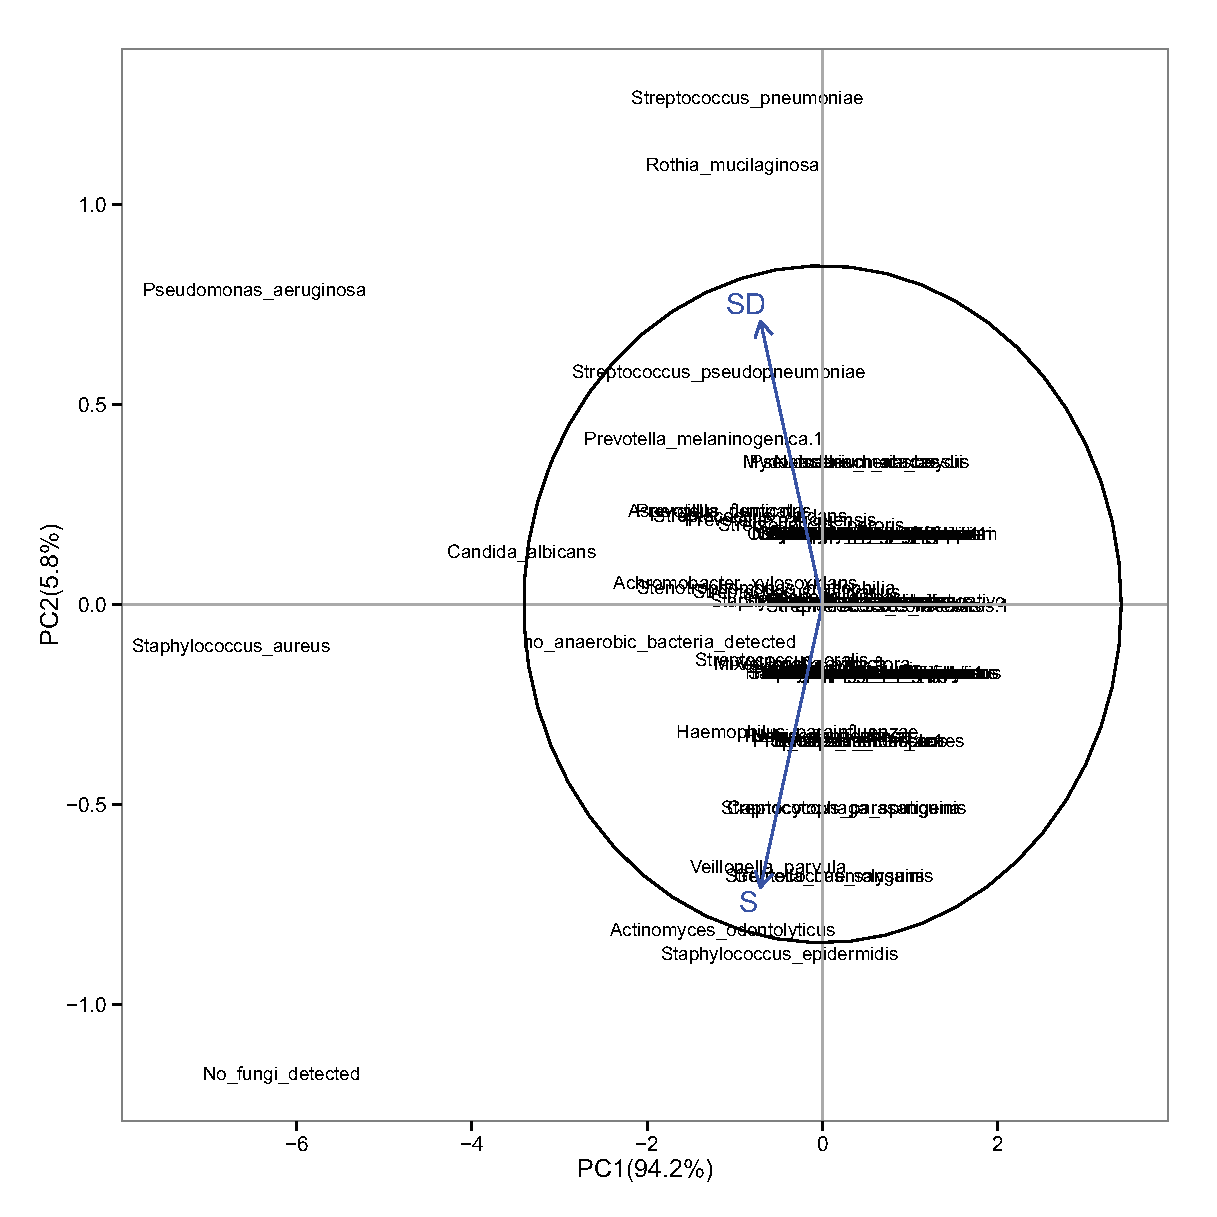
\includegraphics[width=0.8\textwidth]{./figures/Chapter_7/Figure_1_cond_taxa}
  	\caption{\label{fig:fig1condtaxa}Biplot of the principal component analysis of culturable taxa from 78 specimens of stable (S) and substantial decliners (SD) patients with CF. Ellipse with 95\% CI is reported. Numbers on axes indicate the amount of variance explained by each component. Labels outside the 95\% ellipse have been jittered to avoid overlaps.}
\end{figure}
Principal Component analysis (PCA) of the culturable microflora detected from S and SD samples did not reveal any clear distinction between S and SD groups, neither among the three different clinical conditions examined (I, normal/mild lung disease; II, moderate disease; III, severe disease) (Figure S1). Interestingly, when PCA was performed using the detected taxa as centroids, differences in the microbial community composition between S and SD groups were found. Figure~\ref{fig:fig1condtaxa} shows that \textit{Pseudomonas aeruginosa}, \textit{Rothia mucilaginosa}, \textit{Streptococcus pneumoniae, }and \textit{Candida albicans} for SD group, the absence of fungi and \textit{Staphlyoccoccus aureus} for S group are the most important taxa in contributing to variance differences among S and SD patients in our dataset (in terms of taxa outside the confidence ellipse 95\%, which group  the most similarly occurring taxa).\\
\begin{table}
\centering
\scriptsize
\begin{tabular}{l c c}
\hline
a) SD vs. S patients &  & \\		
Taxon & OR & CI 95\% (lower - upper) \\
\hline\hline
Streptococcus pneumonia & \textbf{9.95} & \textbf{1.47 - 233.90} \\
Rothia mucilaginosa & \textbf{4.87} & \textbf{1.03 - 38.80} \\
Pseudomonas aeruginosa & 1.66 & 0.66 - 4.20 \\
Candida albicans & 1.04 & 0.39 - 2.79 \\
Staphylococcus aureus & 0.86 & 0.34 - 2.18 \\
absence of fungi & 0.77 & 0.30 - 1.96 \\
  &  &  \\
b) FEV\textsubscript{1} (III) vs. FEV\textsubscript{1} (I) + (II) &  & \\
Taxon & OR & CI 95\% (lower - upper) \\
\hline\hline
Candida albicans & 1.57 & 0.53 - 4.55 \\
Pseudomonas aeruginosa & 1.46 & 0.40 - 4.94 \\
No anaerobic bacteria & 1.46 & 0.40 - 4.94 \\
\hline
\end{tabular}
\caption{\label{tab:ortrflp}Odds Ratio from culturable microflora with differential occurrence in SD and S patients and FEV\textsubscript{1} groups. Data report the taxa detected from Principal Component Analysis (Figure~\ref{fig:fig1condtaxa}), the Odds Ratio (OR) of association between presence of the taxa and SD status (a) or FEV\textsubscript{1} (III) with respect to a cohort composed by FEV\textsubscript{1} (I) and FEV\textsubscript{1} (II) patients (b), the 95\% confidence intervals (CI 95\%). Statistically significant ORs are reported in bold. FEV\textsubscript{1}, group I = normal/mild (FEV\textsubscript{1}\% {\textgreater} 70); FEV\textsubscript{1}, group II = moderate (70 ${ \geq}$ FEV\textsubscript{1}\% ${\geq}$ 40); FEV\textsubscript{1}, group III = severe (FEV\textsubscript{1}\% {\textless} 40).}
\end{table}
To statistically evaluate the relationships between the differential presence of these taxa and the patients' status, Odds Ratio (ORs) were computed (Table~\ref{tab:ortrflp}). Statistically significant ORs for SD were found for the presence of \textit{S. pneumoniae} (OR=9.954) and \textit{R. mucilaginosa} (OR=4.867) (Table~\ref{tab:ortrflp} (a)). However, taking account the possible confounders in a logistic regression (Table SM3) for \textit{S. pneumonia }OR was 1.12 (CI 0.14-6.11) and \textit{R. mucilaginosa} OR was 7.37 (CI 1.45-44.41). In the same model \textit{P. aeruginosa} OR was 1.14 (CI 0.34-3.87), while \textit{C. albicans, S. aureus }and absence of fungi had ORs of 2.30, 1.04 and 0.57, respectively.\\
\begin{figure}[!tb]
	\centering
	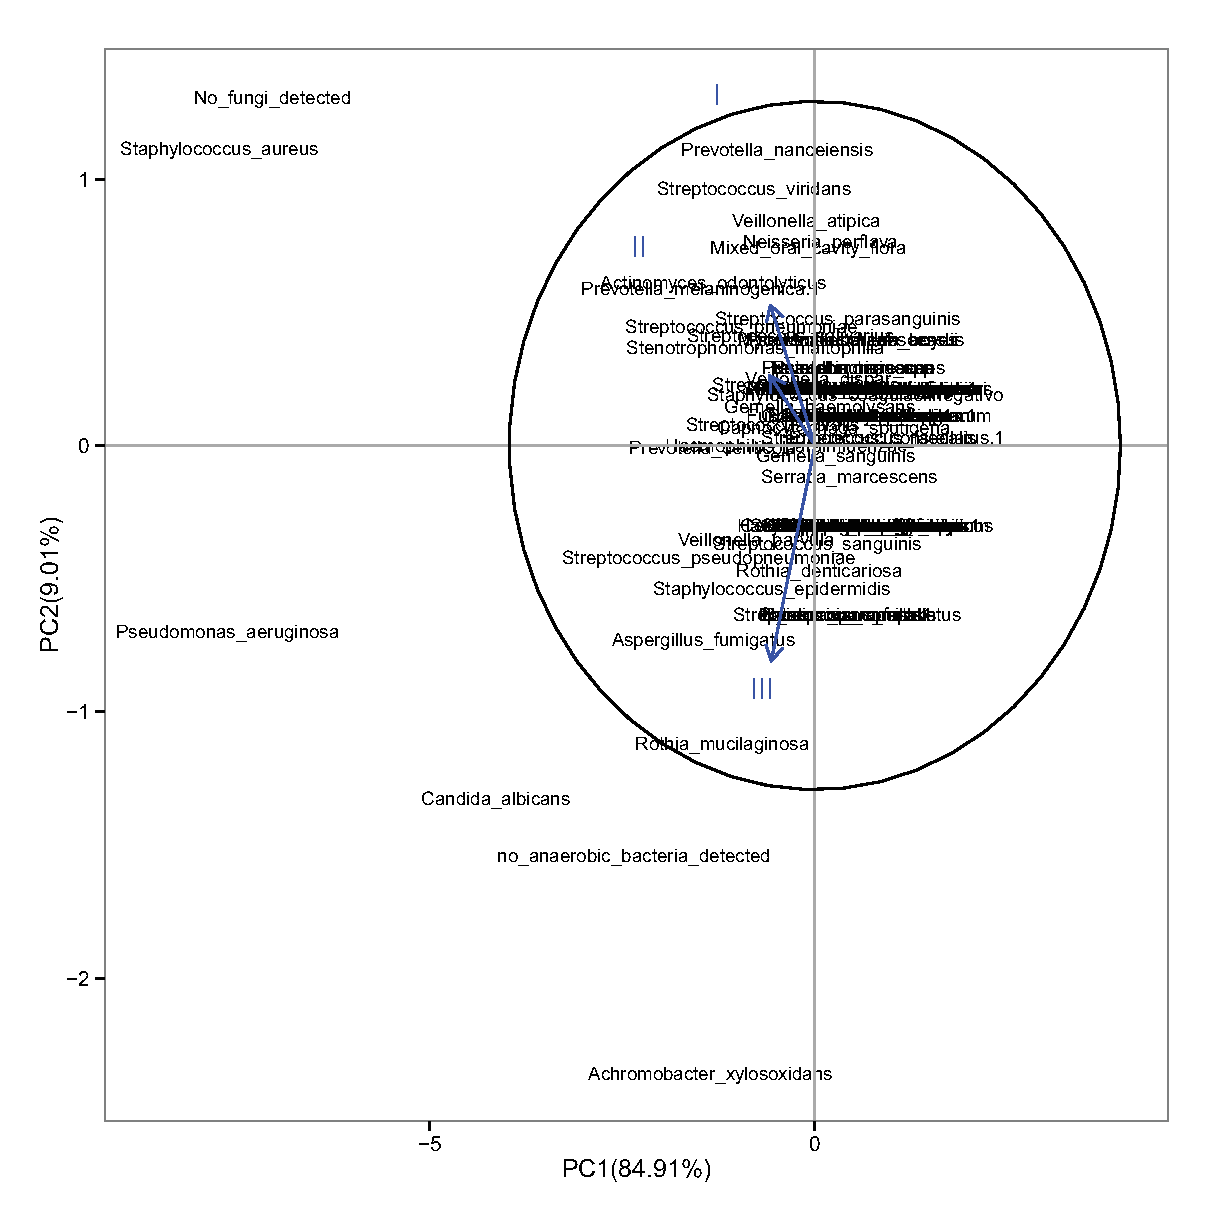
\includegraphics[width=0.8\textwidth]{./figures/Chapter_7/Figure_2_fev1_taxa}
  	\caption{\label{fig:fig2fev1taxa}Biplot of the principal component analysis of culturable taxa from 78 specimens of patients with CF considering their FEV\textsubscript{1} groups. Ellipse with 95\% is reported. Numbers on axes indicate the amount of variance explained by each component. Labels outside the 95\% ellipse have been jittered to avoid overlaps.}
\end{figure}
When the three different FEV{\textsubscript{1}} groups were considered, PCA showed a differential occurrence of \textit{Achromobacter xylosoxidans},\textit{P. aeruginosa},\textit{C. albicans} as well as the absence of an anaerobic microflora in CF patients with severe lung disease (group III) (Figure~\ref{fig:fig2fev1taxa}). Conversely, for the presence of \textit{A. xylosoxidans} no statistical support could be obtained, since this species was detected only in one patient of group III. Considering ORs for the FEV\textsubscript{1} of group III, in comparison with FEV \textsubscript{1} I and II groups (Table~\ref{tab:ortrflp} (b)), no statistically significant ORs were detected between culturable microflora and FEV\textsubscript{1} decline. By applying a logistic regression including confounders the same result was found (Table SM4), with no detectable limit for the lower confidence interval.\\
\begin{table}
\centering
\scriptsize
\begin{tabular}{l c c c}
\hline
Bacterial communities & \multicolumn{3}{c}{Diversity indices} \\
\hline\hline
a) Culturable microflora & Shannon & Evenness & Richness \\
\hline
SD & 1.64 {\textpm} 0.39 & 0.37 {\textpm} 0.06 & 5.6 {\textpm} 2.3 \\
S & 1.65 {\textpm} 0.40 & 0.36 {\textpm} 0.06 & 5.7 {\textpm} 2.4 \\
  &  &  &  \\
b) T-RFLP community profiles &  &  \\
\hline
SD & 1.89 {\textpm} 0.55 & 0.43 {\textpm} 0.18\textsuperscript{a} & 19.8 {\textpm} 11.0 \\
S & 1.86 {\textpm} 0.56 & 0.52 {\textpm} 0.18\textsuperscript{b} & 16.5 {\textpm} 10.8 \\
  &  &  &  \\
c) T-RFLP profiles / FEV\textsubscript{1} groups &  &  \\
\hline
FEV\textsubscript{1} group I & 1.95 {\textpm} 0.49\textsuperscript{a} & 0.45 {\textpm} 0.17 & 19.7 {\textpm} 9.5 \\
FEV\textsubscript{1} group II & 1.59 {\textpm} 0.48\textsuperscript{b} & 0.47 {\textpm} 0.22 & 15.1 {\textpm} 11.9 \\
FEV\textsubscript{1} group III & 2.09 {\textpm} 0.61\textsuperscript{a} & 0.53 {\textpm} 0.15 & 19.6 {\textpm} 11.6 \\
\hline
\end{tabular}
\caption{Diversity estimates for bacterial communities in sputum samples of CF patients. Data show the mean indices for substantial decliners (SD) and stable (S) patients {\textpm} standard deviation. For T-RFLP data, the indices for the three FEV\textsubscript{1} groups are also reported. Different letters indicate statistically significant (P{\textless}0.05) differences after one-way ANOVA and Tukey \textit{post-hoc} comparison.\label{tab:divtrflp}} 
\end{table}
Concerning the overall values of diversity indices, no statistically significant differences in alpha diversity values were found between the whole groups of SD and S patients (Table~\ref{tab:divtrflp} (a)) as well as between SD and S patients belonging to the severe group (FEV\textsubscript{1} group III), and among the three FEV{\textsubscript{1}} sub- roups in both SD and S patients (data not shown). Furthermore, no significant correlation was found between diversity indices and FEV\textsubscript{1} values (as Pearson's r, p value was \textless 0.9 for all indices).\\

\subsubsection{Total microbiota in S and SD CF patients}
\paragraph{Community composition: species absence/presence} In the 78 sputum samples analyzed by T-RFLP, a total of 1411 bands representing 208 different T-RF lengths were detected. The number of individual bands in each sample ranged from 2 to 43. In particular, ranges were from 3 to 43 for the S patients and 2 to 39 for the SD patients. The mean number of T-RF bands per patient in S sample set (20.2 {\textpm} 11.4) was higher than that of the SD sample (15.5 {\textpm} 10.2), though the difference was not significant (P {\textless} 0.06). Among the 208 T-RF bands detected, 82 (39.4\%) were ``singletons'' defined here as bands that occurred in only one sample. Singletons were detected in 18 (45\%) S and 10 (27.2\%) SD samples.\\
\paragraph{Bacterial community structure} PCA carried out on single patient's T-RFLP profiles did not reveal any clear differences between S and SD patients, nor any differences associated with lung disease status (Figure SM1). When PCA was performed on the markers (T-RFs) as centroids, several (16) T-RFs with a differential contribution toward SD and S (as those outside the confidence ellipse at 95\%) were found (Figure~\ref{fig:fig3condtrf}). Identified T-RFs outside the 95\% confidence ellipse in the biplot were putatively assigned to bacterial taxa by \textit{in silico} digestion with \textit{Cfo}I, using the Phylogenetic Assignment Tool (PAT+) provided by Microbial Community Analysis III (MiCA 3) (\href{http://mica.ibest.uidaho.edu/}{http://mica\-.ibest\-.uidaho\-.edu}). Phylogenetic assignment of the T-RFs was grouped at the phylum level.\\ 
\begin{figure}[!tb]
	\centering
	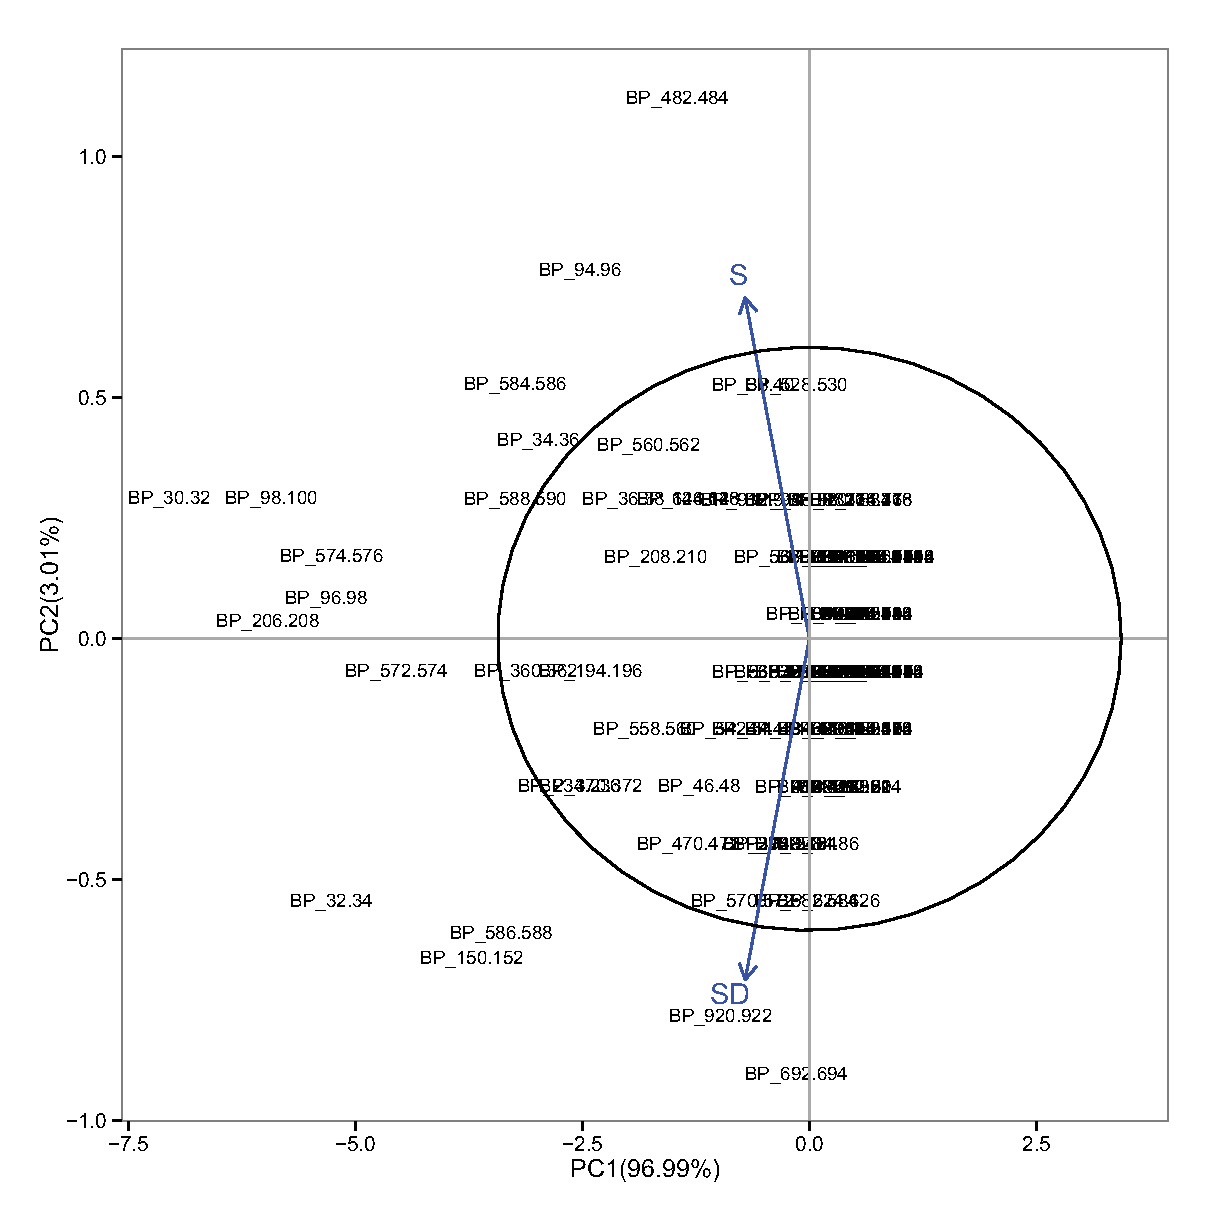
\includegraphics[width=0.8\textwidth]{./figures/Chapter_7/Figure_3_cond_trf}
  	\caption{\label{fig:fig3condtrf}Principal Component Analysis of total occurrences of T-RFs in 78 patients with CF from S and SD patients. Ellipse with 95\% is reported. Comparison of stable with substantial-decliners CF patients. Numbers on axes indicate the amount of variance explained by each component. Labels outside the 95\% ellipse have been jittered to avoid overlaps.}
\end{figure}
One T-RF (920-922 nt) resulted to have a higher impact on the variance of SD status, while another T-RF (482-484 nt) contributed more to the variance of S status. Moreover, the T-RF at 692-694 nt was only detected in SD patients (in eight out of 38 patients, corresponding to approx. 21\%). A query launched on MiCA 3 web server against the database of 16S rRNA gene sequences allowed to putatively assign 10 out the above mentioned 16 T-RFs to known bacterial taxa. To statistically evaluate the relationships between the differential presence of these taxa and the patients' status, ORs were computed for TFs, too (Table~\ref{tab:ordettrflp}). In particular, T-RFs with OR {\textgreater} 1 (Table~\ref{tab:ordettrflp} (a), i.e., more present in SD than in S patients) enabled to detect \textit{Pseudomonas}, \textit{Shewanella}, and \textit{Burkholderia}. Interestingly, a T-RF putatively assigned at \textit{Shewanella - Colwellia} (920-922 nt) resulted with a high OR for SD patients. The logistic regression model was well in agreement with CMLE ORs estimates (Table SM5). However, several T-RFs were not assigned to any known cultured taxon nor can be assigned to any 16S rRNA gene sequence present in the database (unidentified), including the T-RF at 482-484 nt which is indicated as more frequent in S patients (OR {\textless} 1).\\
\begin{table}
\centering
\tiny
\begin{tabular}{l c c l}
\hline
TRF size (nt) & OR & CI 95\% (lower - upper) & Putative taxonomic attribution \\
\hline\hline
a) SD vs S &  &  &  \\	
\hline
30-32 & 0.94 & 0.26 - 3.39 & Burkholderia \\
32-34 & 2.05 & 0.79 - 5.51 & Burkholderia, Streptomyces \\
34-36 & 0.79 & 0.31 - 1.98 & Anaerofilum, uncultured \\
94-96 & 0.56 & 0.21 - 1.43 & Chloroflexi, Bacteroidetes, uncultured \\
96-98 & 0.28 & 0.06 - 1.06 & Pseudoalteromonas, uncultured \\
98-100 & 0.93 & 0.33 - 2.64 & Cycloclasticus, Mannheimia, uncultured \\
150-152 & 2.04 & 0.83 - 5.15 & uncultured \\
206-208 & 1.18 & 0.44 - 3.17 & Pseudomonas, uncultured \\
482-484 & \textbf{0.29} & \textbf{0.08 - 0.88} & unidentified \\
572-574 & 1.25 & 0.50 - 3.13 & Pseudomonas, Shewanella \\
574-576 & 1.04 & 0.40 - 2.68 & Shewanella \\
584-586 & 0.72 & 0.29 - 1.79 & uncultured \\
586-588 & 2.04 & 0.83 - 5.15 & unidentified \\
588-590 & 0.89 & 0.36 - 2.20 & unidentified \\
692-694 & n.d. & n.d. - n.d. & unidentified \\
920-922 & 3.61 & 1.06 - 14.37 & Shewanella, Colwellia \\
 &  &  & \\
b) FEV\textsubscript{1} (III) vs FEV\textsubscript{1} (I)+(II) &  &  \\
\hline
208-210 & 2.36 & 0.84 - 6.74 & Pseudomonas \\
194-196 & 2.55 & 0.96 - 6.87 & uncultured \\
234-236 & 2.09 & 0.80 - 5.52 & unidentified \\
572-574 & 2.11 & 0.81 - 5.77 & Pseudomonas, Shewanella \\
96-98 & \textbf{3.00} & \textbf{1.00 - 10.18} & Pseudoalteromonas, uncultured \\
574-576 & 2.15 & 0.78 - 6.34 & Shewanella \\
586-588 & 1.50 & 0.59 - 3.86 & unidentified \\
360-362 & 1.47 & 0.57 - 3.77 & uncultured \\
98-100 & 2.10 & 0.68 - 7.23 & Cycloclasticus, Mannheimia, uncultured \\
206-208 & 1.66 & 0.59 - 4.94 & Pseudomonas, uncultured \\
32-34 & 1.01 & 0.38 - 2.73 & Burkholderia, Streptomyces \\
30-32 & 1.22 & 0.33 - 5.06 & Burkholderia \\
34-36 & 0.70 & 0.26 - 1.83 & Anaerofilum, uncultured \\
560-562 & 0.36 & 0.11 - 1.09 & Cellvibrio, Pseudomonas, uncultured \\
470-472 & 0.40 & 0.10 - 1.33 & uncultured \\
558-560 & \textbf{0.28} & \textbf{0.07 - 0.90} & Halomonas \\
144-146 & \textbf{0.07} & \textbf{0.00 - 0.42} & uncultured \\
150-152 & \textbf{0.25} & \textbf{0.09 - 0.66} & uncultured \\
\hline
\end{tabular}
\caption{\label{tab:ordettrflp} Odds ratio from TRFs with differential occurrence in S and SD patients and FEV\textsubscript{1} groups. Data report the TRFs size in nucleotides (nt), the CMLE Odds Ratio (OR) estimates of association between presence of the TRF and SD status (a) or FEV\textsubscript{1} (III), the 95\% confidence intervals (CI 95\%) and the putative taxonomic attributions with MiCA web server. The reported attributions indicate the main hits retrieved for that particular size. Statistically significant ORs are reported in bold.} 
\end{table}
PCA biplot (Figure~\ref{fig:fig4fev1trf}) showed that the vector of FEV\textsubscript{1} group I has a different orientation with respect to those of the other FEV textsubscript{1} groups, suggesting that some T-RFs can indeed be differentially present. We then computed ORs for the 18 T-RFs outside the ellipse 95\%. Results are reported in Table~\ref{tab:ordettrflp} (b). One T-RF (96-98 nt) resulted to contribute more to the variance of FEV\textsubscript{1} group III, while three T-RFs (558-560 nt, 144-146 nt, 150-152 nt) contributed more to the variance of FEV\textsubscript{1} I and II groups. Putative taxonomic identification carried out on such T-RFs highlighted that most of them cannot be assigned (as uncultured or unidentified). The T-RF at 558-560 nt can indeed be assigned to \textit{Halomonas}. However, though CMLE ORs (Table~\ref{tab:ordettrflp} (b)) showed significant ORs the logistic regression model (Table SM6) did not show supported the data.\\
\begin{figure}[!tb]
	\centering
	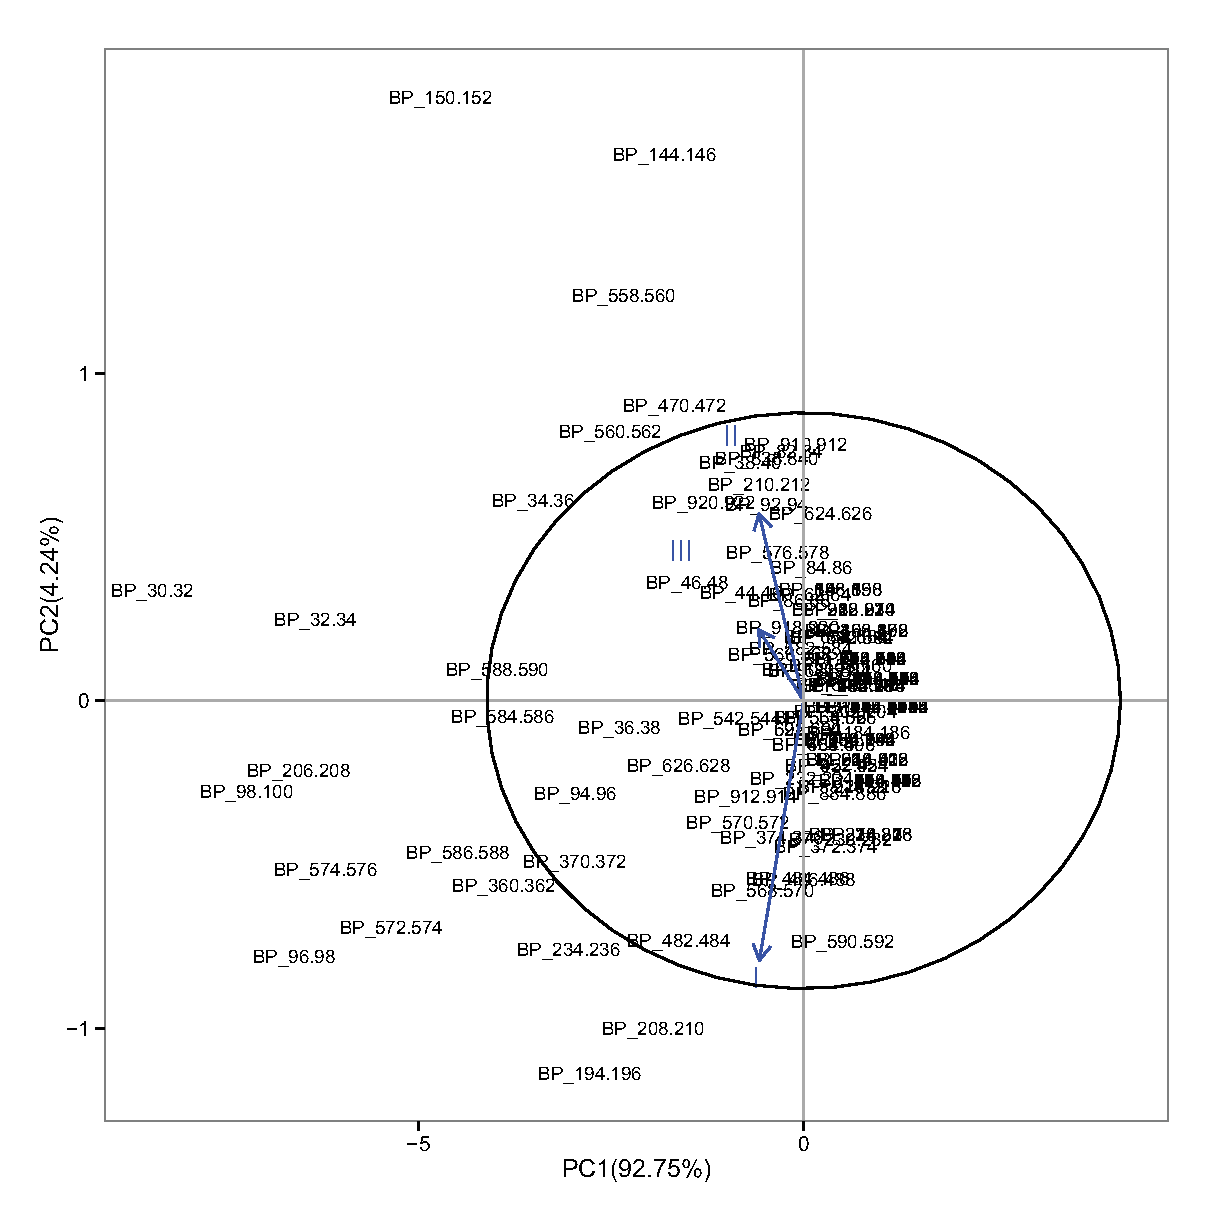
\includegraphics[width=0.8\textwidth]{./figures/Chapter_7/Figure_4_fev1_trf}
  	\caption{\label{fig:fig4fev1trf} Principal Component Analysis of total occurrences of T-RFs in 78 patients with CF from S and SD patients. Ellipse with 95\% is reported. Comparison among FEV\textsubscript{1} groups (I, II, III). Numbers on axes indicate the amount of variance explained by each component. Labels outside the 95\% ellipse have been jittered to avoid overlaps.}
\end{figure}

\paragraph{Diversity indices} To investigate changes in bacterial communities that may have occurred with severe decline in lung function, diversity indices were computed for all samples by using community ecology parameters (beta diversity estimates). Results revealed that the Evenness, i.e. the equal distribution of T-RFs, resulted higher in S sample set (0.52 {\textpm} 0.18) than in SD sample set (0.43 {\textpm} 0.18) (p {\textless} 0.05). The other diversity indices considered (Richness and Shannon) were not statistically different between the whole dataset of S and SD patients (p {\textgreater} 0.05) (Table~\ref{tab:divtrflp} (b)), and no statistically significant changes were observed between S and SD groups when considering the three FEV\textsubscript{1} sub-groups separately (data not shown). The diversity indices (Evenness, Richness) values did not allow to detect differences among the three FEV textsubscript{1} groups (Table~\ref{tab:divtrflp} (c)), while significant (p{\textless}0.05) differences in Shannon indices of FEV\textsubscript{1} (II) \textit{vs} FEV\textsubscript{1} (I) and of FEV\textsubscript{1} (II)\textit{vs} FEV textsubscript{1} (III) were found. However, no significant differences were found for FEV\textsubscript{1} (I) \textit{vs} FEV\textsubscript{1} (III).\\

\subsection{Discussion}
In the present study, we used both culture-dependent methods for detection of aerobic and anaerobic bacteria and fungi, and a culture-independent method by terminal restriction fragment length polymorphism (T-RFLP), which provide a fingerprint of the most highly abundant members of the community. Data presented here provide new insights into the CF airway microbiota of S and SD patients, population dynamics of the microbiota following lung disease status (normal/mild, moderate and severe lung disease), ecology of the bacterial communities related to lung function decline and establishment of specialized communities of pathogens associated with poor pulmonary function, including putative discriminant microbial species and T-RFs for S and SD groups.\\
The percentage predicted forced expiratory volume in 1 s (FEV\textsubscript{1}\%) is currently the gold standard measure of disease severity in patients with CF. The rate at which FEV\textsubscript{1} declines over a period is an indicator of aggressiveness of a patient's lung disease, regardless of the stage of the patient's lung disease (normal/mild, moderate and severe) \cite{zhao2012decade}. In the present work, we defined as a substantial decline in lung function a decrease of 5\% or more in FEV\textsubscript{1} predicted per year. This percentage drop in FEV\textsubscript{1} suggests a substantial decline similar to that defined by Vandenbranden and colleagues \cite{vandenbranden2012lung} and twice the one reported in published studies \cite{sanders2010failure}. Therefore, the microbiota investigation in CF patients with a more substantial decline in lung function over the previous year can be very useful in order to try to understand where a pathogen is only a marker of disease severity or an independent contributor to the loss of lung function \cite{milla1998risk}.  As ultimately the goal of pulmonary interventions is to retard the disease process and therefore reduce the rate of lung function decline, defining new potential biomarkers for the early detection of severe rate of decline in lung function could be essential for making rational decisions regarding intervention.\\
The presence of \textit{P. aeruginosa} in respiratory tract cultures has been previously reported to be associated with a more rapid decline in lung function, especially when mucoid phenotype is present \cite{emerson2002pseudomonas}. However, Vandenbranden and colleagues \cite{vandenbranden2012lung} found that the presence or absence of \textit{P. aeruginosa} or mucoid \textit{P. aeruginosa} was not predictive of lung function decline. Our findings from culture-based analysis showed that \textit{P. aeruginosa} cannot be strongly proposed as indicative of severe decline in lung function (OR = 1.14, CI 0.34-3.87). It is noteworthy that maintenance treatment for chronic \textit{P. aeruginosa} with inhaled antibiotics and/or azithromicin in accordance with the Guidelines \cite{farrell2008guidelines}. resulted in slowing down the rate of decline in FEV\textsubscript{1}. Our culture-based results suggest an important role of \textit{S. pneumoniae} and \textit{R.mucilaginosa} as marker species for SD status. Although \textit{S.pneumoniae} is a common respiratory tract pathogen, it is unusual in CF \cite{foweraker2009recent}. This bacterial species is able to persist in the CF lung and has been recently regarded as pathogenic within the CF community \cite{maeda2011population}. However, to the best of our knowledge, it is still unclear whether \textit{S.pneumoniae} has a role in acute exacerbation and severe lung decline or can act synergically with other CF pathogens. As regards \textit{R. mucilaginosa}, it was previously reported as an aerobic species isolated from CF sputum \cite{tunney2008detection} and it was defined by several Authors \cite{bittar2008molecular} as a ``new'' emerging CF pathogen. Recently, Lim and colleagues \cite{lim2013mechanistic} confirmed that \textit{R. mucilaginosa} is present and metabolically active in the lungs of CF patients and that it evolves and adapts to each patient's lung environment over the course of a persistent infection. Our results also reinforce the previous findings of Chotirmall and colleagues \cite{chotirmall2010sputum} who reported that colonization with \textit{C. albicans} presages FEV\textsubscript{1} decline in CF. Although the same Authors suggested the implication of \textit{C. albicans} in the decline of CF lung function, the clinical relevance of yeasts is still a matter of debate, and has yet to be confirmed. Our findings add support to $i)$ the pathogenicity of species derived from the oral cavity and usually considered as clinically insignificant, and $ii)$ the complex interaction between typical pathogens and microbiota, such as the association between \textit{P. aeruginosa} and anaerobes/fungi.\\
It is well known that CF airways harbor numerous organisms that evade detection by culture-based methods. To carefully examine the microbiota from patients with stable versus worsening disease status, we chose to utilize T-RFLP analysis to generate community profiles. T-RFLP is a popular molecular profiling technique with the capacity to resolve community members based on the position of restriction sites in the 16S rRNA gene \cite{liu1997characterization}. T-RFLP profiles have been extensively used for community differentiation, identification of specific organisms in microbial populations  and comparison of the relative phylotype richness and community structure in a diverse range of environments \cite{osborn2000evaluation, marsh2005culture, tiquia2010using, joo2010monitoring, nakano2010prediction}. When previously applied to the analysis of spontaneously expectorated sputum from CF patients, T-RFLP has indicated the presence of a diverse array of bacterial species \cite{stressmann2011analysis, rogers2010determining, rogers2003bacterial, sibley2008polymicrobial}. In this study, we used T-RFLP analysis as a tool to investigate two key topics. First, do the bacterial communities (microbiota) detected in S samples differ from those in SD samples? Additionally, are there differences in the microbiota among CF patients with different status of lung disease? Results obtained in the present study by T-RFLP analysis revealed a greater bacterial diversity within sputum samples than that detected by culture approaches. We did not find T-RFLP profiles exclusive of the patients from S or SD groups. T-RFLP analysis revealed sixteen T-RFs as the most differentiating between S and SD groups after PCA. However, in our dataset, significant ORs were only recorded for two of them (and only one was possible to identifiy as putative \textit{Shewanella})Interestingly, the other T-RFs which differentiate (tough not significantly on the basis of ORs) S from SD were putatively identified as belonging to known CF pathogens, as \textit{Pseudomonas} and \textit{Burkholderia}, but most of them resulted in no species assignation (only {\textasciitilde}18\% of T-RF band lengths match a band length generated from published sequence data).Therefore, these unknown T-RFs could be either novel species or related species/strains of the core community of CF airways, but with enough heterogeneity in the 16S rRNA gene that may generate slightly different fragment sizes \cite{camarinha2012validating}. \textit{S.pneumonia} and \textit{R. mucilaginosa} were detected by culturing but not by T-RFLP analysis. It is well known that molecular methods based on 16S sequence data have a limited ability to resolve taxonomic identification at the species level \cite{filkins2012prevalence} and may introduce biases during the primer-binding step of PCR \cite{cai2013biased}. In spite of these limits, and taking also into consideration that T-RFLP only allows a putative (though fast) taxonomic assignment, this culture-independent method adds valuable information to the data obtained from culture analysis. To gain a more comprehensive characterization of CF lung microbial communities, more sophisticated and expensive techniques, such as bacterial metabarcoding by 16S rDNA and metagenomic sequencing \cite{maughan2012analysis, lim2014clinical} will be applied. \\
To investigate changes in bacterial communities that may have occurred with substantial decline in lung function, the diversity indices on T-RFLP data were calculated for all samples. Diversity provides a measure of community complexity based on the number (Richness) and relative abundances (Evenness) of the species present. The reduced Evenness observed in SD respect to S group of patients revealed an impaired ecology of the bacterial community in SD patients, which in turn can be associated with lung function decline experienced by those patients. When we assessed community structures to describe the degree of change occurring in the airway microbiota following the decline in lung function, we did not find a decrease in Shannon diversity index with advanced disease in the SD group. As suggested by Zhao and colleagues \cite{zhao2012decade}, other factors, such as antibiotic use, rather than lung function or patient age have been found to be the primary drivers of the decreasing bacterial diversity in CF patients with progressive lung disease. In our study, patients with a more rapid decline in lung function did not have a higher antibiotic exposure over the previous year with respect to S patients; additionally, both S and SD patients did not receive antibiotics in the 30 days preceding the specimen collection. Collectively, our results suggest that the antibiotic use is not likely to have contributed to the failure in detecting a decrease in community diversity with advanced disease in the SD group. Moreover, we cannot \textit{a priori} exclude that the use of relative peak intensities as a proxy for taxa frequency, though largely used (for instances see  \cite{camarinha2012validating, blackwood2007interpreting, ding2013community}), may be someway biased and can produce altered data. Our analyses suggest that overall bacterial diversity remains relatively stable despite the decreasing in relative abundances of the species in SD patients. Indeed, as previously stated by Zhao and colleagues \cite{zhao2012decade}, community diversity alone is not a sufficient indicator of the disease status. However, considering only the three subgroups of FEV\textsubscript{1} (normal/mild \textit{vs} moderate, \textit{vs} severe), independently from the rate at which FEV textsubscript{1}\% declines, statistically significant differences among the three sub-groups were also found, suggesting that the patients with intermediate FEV\textsubscript{1} values are experiencing changes in the airway assembly of taxa. A more detailed taxonomic and functional analysis of the microbial community of lung microbiota of CF patients could help elucidating the microbial factors that can contribute to such changes.\\ 
In conclusion, by combining culture-dependent and culture-independent methods with ecological tools and clinically relevant information, a more comprehensive view of microbial community composition in SD patients with CF was determined. Overall, our results suggest that the presence of \textit{P. aeruginosa} ``per se'', as well as the single T-RFLP profiles, are not able to define the S or SD group. New biomarkers are required in CF to predict the decline clinical phenotype and monitor the response of CF patients to existing and new therapeutic strategies. Microbial factors represent a potential to provide biomarkers for the early detection of the substantial lung function decline in CF. We have identified some discriminatory species as well as some discriminatory T-RFs, that represent good candidates as predictors of substantial decline in lung function, enabling to stratify individuals with CF at high or low risk of future severe lung function decline. However, only longitudinal studies can help determine patterns of association between the CF airway microbiome and lung disease. A more in-depth investigation of microbial airway bacterial communities in longitudinal studies and by high-throughput sequencing and bioinformatics tools will provide powerful means to better understand the contribution of the airway microbiome to severe decline in FEV\textsubscript{1} and its potential for the development of new biomarkers as predictors of severe pulmonary disease in CF patients.\\

\subsection{Acknowledgements} We thank John LiPuma, Gianni Mastella and late Gerd D\"oring for their helpful suggestions. We dedicate the present article to the memory of Gerd D\"oring (University of T\"ubingen, T\"ubingen, Germany), who was a world authority on infection and inflammation in the CF lung. With Gerd's death, we lost an excellent scientist, a loyal and generous friend, a marvelous speaker, and a charming person of great sensitivity and nobility. We also acknowledge the Italian Cystic Fibrosis Research Foundation (FCC) for its support and administrative tasks, and Graziana Manno, Anna Marchese, Silvia Campana, Gabriella Ricciotti, Cristina Cantale for their valuable assistance. \\

%%%%%%%%%%%%%%%%%%%%%%%%%%%%%%%%%%%%%%%%%%%%%%%%%%%%%%%%%%%%%%%%%%%%%%%%%%%%%%%%%%%%%%%%%%%%%%%%%%%%%%%%%%%%%%%%%%%%%%%%%%%%%%%%%%%%%%%%
%%%%%%%%%%%%%%%%%%%%%%%%%%%%%%%%%%%%%%%%%%%%%%%%%%%%%%%%%%%%%%%%%%%%%%%%%%%%%%%%%%%%%%%%%%%%%%%%%%%%%%%%%%%%%%%%%%%%%%%%%%%%%%%%%%%%%%%%

\section{Taxonomic signatures of CF airway microbiota distinguish between stable and severe declining patients}
Cystic fibrosis (CF) is an autosomal recessive genetic disorder characterized by a progressive decline in lung function. Patients with CF may show a rapid and severe decline of their pulmonary efficiency, measured as FEV\textsubscript{1} percentage, despite antibiotic treatment. Usually, these treatments are selected relying on the susceptibility of individual and culturable microbial strains to specific antibiotics in vitro. Nevertheless, this approach may not correctly predict medical outcomes because of both technical and biological factors. In these years, several culture-independent studies have shown that the CF airway infection is significantly more complex and dynamic than previously detected. Thus, understanding the ecological and evolutionary dynamics able to modify the lung microbiota of CF patients is critically important for either developing new and more effective therapies or improving existing ones. In this study, we analyzed the sputum from 52 patients with different disease conditions through 16S rRNA metabarcoding analysis in order to bring an in-depth overview of the lung microbiota at different stages of CF disease. The enrolled patients were divided into 2 main groups based on their rate decline in FEV\textsubscript{1} value per year. Patients with a rate decline greater than -1.5\% were assigned to the ``stable'' group (S), whereas patients with a rate decline between -1.5\% and -5.0\% were assigned to the ``severe decliners'' group (SD). Moreover, patients were further categorized into three FEV\textsubscript{1} groups: group I (FEV\textsubscript{1} {\textgreater} 70\%); group II (FEV\textsubscript{1} ranging from 40\% to 69\%) and group III (FEV\textsubscript{1} {\textless} 40\%). Surprisingly, the metabarcoding analysis has shown that bacterial biodiversity of stable patients dropped down passing from group I to group II of FEV\textsubscript{1} index; whereas bacteria community connection has a similar behavior passing from ``stable'' to ``severe decliners conditions''. Here, we theorize that something (still unknown) is occurring in the ecology of lung microbiota passing from FEV\textsubscript{1} I to FEV\textsubscript{1} II, which may misbalance bacterial community ecology, opening the way to more severe conditions.\\

\subsection{Introduction}
The main goal of pulmonary interventions is to retard the disease process reducing the rate of lung function decline even defining new potential biomarkers for the early detection of severe rate of decline in lung function, essential for taking rational decisions regarding intervention.\\
In recent years the microbial ecology of the airways in cystic fibrosis (CF) has been shown to be significantly more complex than originally considered \cite{lipuma2010changing, rogers2014respiratory}. Recent works using culture-independent identification methods have revealed that CF patients harbor a vast array of bacteria, previously not identified and not suspected to be involved in the infection and inflammation typical of CF patients \cite{zhao2012decade}. During the last few years, the development of next-generation sequencing technologies and bioinformatics tools has enabled the large-scale investigation of microbial communities and has facilitated our understanding of a ``black box'' of microbial communities present in CF airways \cite{delmont2011metagenomic}. These findings have altered drastically our understanding of CF lung disease \cite{rogers2014respiratory}, but their translation into improvements in clinical outcome remains a substantial obstacle to improving the quality of care. It has been proposed that the lung microbial communities might be considered as a unique distinct pathogenic entity, whose impact on the host may be greater than the combined impacts of its individual component species alone \cite{rogers2010comparing}. Indeed, an ecological perspective on multispecies colonization of the CF airways will permit to understand the role of polymicrobial dynamics in CF lung disease and provide the clinicians with new biomarkers of CF progression, as well as with new bacterial targets for antibiotic treatment \cite{sibley2008polymicrobial}.\\
Until now, many efforts have been made to identify microbes associated with airway diseases, antibiotic treatment, patient age increasing, and periodic pulmonary exacerbation \cite{zhao2012decade, cox2010airway, carmody2013changes, zhao2014modeling, zemanick2013inflammation}. However, it is still not clear how changes in the airway microbiota composition are predictive of severe lung disease progression. Bacterial infections in the CF airways are currently monitored through routine microbiology and CF patients receive cures based on culturable microbial pathogens colonizing their airways \cite{flume2009cystic}. It has been found that the administration of antimicrobial therapy, based on the in vitro susceptibilities of classic CF pathogens, does not necessarily correlate with the clinical outcome \cite{sibley2009relevance}.\\
Here we used 16S rRNA metabarcoding analysis of lung microbiota to describe the ecological issues (biological diversity, taxa composition, interaction among taxa) related to a specific pulmonary physiopathological status. We analyzed the microbiota of a large cohort of patients (a total of 52 patients) differing for status (S and SD) and FEV\textsubscript{1} index values in order to explore how bacterial communities change during the course of CF disease.\\

\subsection{Materials and Methods}

\subsubsection{Ethics Statement}
Sputum samples from patients with CF were collected at Bambino Ges\`u Children's Hospital (Rome, Italy), Cystic Fibrosis Center, Meyer Children's Hospital (Florence, Italy) and Giannina Gaslini Children's Hospital (Genoa University, Genoa, Italy), in accordance with the ethical guidelines. The study was approved by the local Ethics Committee of each participating Center [Prot. 85 of February 27, 2014 (Meyer Children's University Hospital); Prot. n. 681 CM of November 2, 2012 (Bambino Ges\`u Children's Hospital); Prot. n FCC 2012 Partner 4-IGG of September 18, 2012 (Giannina Gaslini Institute)]. Informed written consent was obtained from all subjects aged 18 years and over and from parents of all subjects under 18 years of age prior to enrollment in the study. The study protocol was in accordance with the Guidelines of the European Convention of Human Rights and Biomedicine for Research in Children and to those of the Ethics Committees of Bambino Ges\`u, Meyer and Giannina Gaslini Hospitals. All measures were taken to ensure patient data protection and confidentiality.\\

\subsubsection{Patients}
52 patients attending three Italian CF Centers (Bambino Ges\`u Children's Hospital, Rome; CF Center, Meyer Children's Hospital, Florence; and Giannina Gaslini Children's Hospital, Genoa) were enrolled in the study between September 2012 and April 2013. Patients, who had been diagnosed with CF according to the published Guidelines \cite{farrell2008guidelines}, were treated by following such Guidelines and consensus for lung monitoring with at least four microbiological controls per year \cite{flume2009cystic}. Patients were eligible if they could be classified as clinically stable, without any pulmonary exacerbation and antibiotic e.v. or oral therapy in the previous 4 weeks \cite{fuchs1994effect, ramsey1999intermittent}.\\
The annualized rate of FEV\textsubscript{1} decline was used to stratify patients as previously reported. CF patients were categorized as ``stable'' (S), i.e. with a rate decline in FEV\textsubscript{1} value no greater than -1.5\% per year, and with a ``substantial decline'' (SD) in FEV\textsubscript{1}, i.e. a rate of FEV\textsubscript{1} decline greater than - 5\% predicted per year. Both S and SD patients were further categorized in three FEV\textsubscript{1} groups: group I, CF patients with normal lung function or mild lung disease (FEV\textsubscript{1} {\textgreater} 70\%); group II, CF patients with a moderate lung disease (FEV\textsubscript{1} ranging from 40\% to 69\%); group III, CF patients with a severe lung disease (FEV\textsubscript{1} {\textless} 0\%). FEV\textsubscript{1} values were measured according to the American Thoracic Society-European Respiratory Society standards \cite{miller2005standardisation}. The overall description of the patient dataset is reported in Table SM1. For additional details on patients number and the number of sequences generated for each group of patients see Table~\ref{tab:ffc116s}.\\
\begin{table}
\centering
\scriptsize
\begin{tabular}{c c c c}
\hline
FEV1 & Condition & \# Patients & \# Sequences \\
\hline\hline
I & S & 13 & 35746 \\
II & S & 10 & 29462 \\
III & S & 6 & 19499 \\
I & SD & 10 & 31332 \\
II & SD & 7 & 20121 \\
III & SD & 6 & 21947 \\
Total &  & 52 & 158107\\
\hline
\end{tabular}
\caption{\label{tab:ffc116s}Number of enrolled patients in each group. The table reports also the number of amplicon sequences assigned to each group.} 
\end{table}

\subsubsection{Sample processing and DNA extraction} 
The analysis of the bacterial community composition was performed on spontaneously expectorated sputum (SES) samples since sputum specimen represents by far the most widely used sample in productive patients \cite{rogers2010comparing}. Samples processing was performed as previously described. About 400 {\textmu}l aliquots of frozen sputum were subjected to genomic DNA extraction using the commercially-available Kit QIAamp DNA Mini Kit. Sample aliquots were spun at 10,000{\texttimes}g to pellet cellular material. After removal of the supernatant, cell pellets were resuspended in 180 {\textmu}l of enzyme solution (20 mg/ml lysozyme in 20 mM Tris{\textperiodcentered}Cl, pH 8.0, 2 mM EDTA, 1.2\  Triton), incubated for 30 min at 37{\textdegree}C and then processed according to the manufacturer's protocol. Quantity and purity of extracted DNA were checked by NanoDrop (NanoDrop Technologies, USA) and PicoGreen fluorescent assay (Life Technologies) and gel electrophoresis.\\

\subsubsection{Amplification and barcoding of bacterial 16S rRNA gene amplicons}
Fifty-four samples (from 52 patients) were obtained and subjected to 16S rRNA gene amplification. The V3, V4, and 5 hypervariable regions of the 16S rRNA gene were amplified using primer 357F (5'-CTA\-CGG\-GAG\-GCA\-GCA\-G-3') modified with the addition of the 454 FLX-titanium adaptor ``B'' sequence (5'-CTA\-TCC\-CCT\-GTG\-TGC\-CTT\-GGC\-AGT\-CTC\-AG-3') and primer 926R (5'-CCG\-TCA\-ATT\-CMT\-TTR\-AGT-3') modified with the addition of 18 unique seven-nucleotide barcode sequences (MID 1 - MID 18, Roche MID adapters) and the 454 FLX titanium adaptor ``A'' sequence (5'-CCA\-TCT\-CAT\-CCC\-TGC\-GTC\-CAT\-CTC\-ATC\-CCT\-GCG\-TGT\-CTC\-CGA\-CTC\-AG-3').\\
Primer design and barcode sequences were as previously reported by Human Microbiome Project (HMP) Consortium \href{http://www.hmpdacc.org/tools\_protocols/tools\_protocols.php}{http://\-www\-.hmp\-dacc\-.org/\-tools\_proto\-cols/\-tools\_pro\-to\-cols\-.php}.\\
PCR amplification was performed on 30 {\textmu}g of DNA template in a total volume of 25 {\textmu}L containing 1{\texttimes} AccuPrime Buffer II (Life Technologies), 10 {\textmu}M of 357F fusion-primer, 10 {\textmu}M of 926F fusion-primer and 0.03 U/{\textmu}L AccuPrime High-Fidelity \textit{Taq} DNA polymerase (Life Technologies). PCR reactions were heated at 95 {\textdegree}C for 2 min followed by 30 cycles of 95 {\textdegree}C for 20 s, 55 {\textdegree}C for 30 s, and 72 {\textdegree}C for 5 min. All reactions were prepared in a sterile PCR hood. Three independent 25 {\textmu}L PCR reactions were generated for each patient DNA-template. Negative control reaction (no DNA template) were also performed. 2.5 {\textmu}L of each replicate reactions were examined by electrophoresis on an 1,5 \% agarose gel. PCR amplicons were cleaned using the Agencourt AMPure XP Beads according to the manufacturer's specifications (Beckman Coulter). To ensure removal of primers and any nonspecific amplicons, purified amplicon libraries were analyzed using the Agilent Bioanalyzer 2100 employing the Agilent DNA 1000 Kit. The concentration of the purified amplicons was determined using the Quant-iT PicoGreen dsDNA fluorescent assay Kit (Life Technologies).\\
For each patient sample, the three independent purified and quantified PCR reactions were pooled in an equimolar ratio of 109 molecules {\textmu}l-1. Amplicon pools were quantified using KAPA Library Quantification Kits (KAPA Biosystems) to determine exactly the number of amplifiable molecules in the amplicon libraries. For 16S Amplicon qPCR reactions two dilutions (1:500 and 1:1000) of each purified library were used. qPCR amplification was performed on 4 {\textmu}L of Amplicon library template in a total volume of 10 {\textmu}L containing 6 {\textmu}L of KAPA SYBR{\textregistered} FAST qPCR Master Mix. Reactions were heated at 95 {\textdegree}C for 5 min followed by 35 cycles of 95 {\textdegree}C for 30 s, and 60 {\textdegree}C for 90 s. In addition, dissociation (melt curve) analysis was performed to provide indication of possible primer- and/or adaptor-dimer contamination of libraries.\\ The concentration of each Amplicon library in molecule/{\textmu}L was achieved by inference from a standard curve generated using the six DNA Standard included in KAPA Library Quantification Kits.\\

\subsubsection{Amplicon Library Amplification and Pyrosequencing} 
To clonally amplify the amplicon libraries, the optimal amount of DNA to use in emPCR amplification was determined using emulsion titration procedure according to the supplier's instructions described in ``emPCR Amplification Manual'' (454 Life Sciences Roche Corporation). Before emulsion titration, MID-containing libraries (MID1 to MID18) were normalized to the same molecule concentration, pooled in equal volumes, and diluted to the emulsion PCR working concentration according to the supplier's instructions described in ``emPCR Amplification Manual'' (454 Life Sciences Roche Corporation). Overall, 3 equimolar amplicon library pools were prepared and purified with AMPure XP beads. Emulsion PCR, emulsion breaking and amplicon pyrosequencing were performed applying the 454 GS FLX+ chemistry following supplier protocols (454 Life Sciences Roche Corporation). Sequencing of amplicons was conducted on a 454 GS FLX+ System (454 Life Sciences Roche Corporation); each of the 3 amplified amplicon libraries was loaded on a PicoTiterPlate (PTP) device, using 3 regions of a medium regions ``4-lane'' gasket. The latest GS FLX+ software 2.9 version was used to sequencing and the pipeline 3 for long amplicon was used to data processing (454 Life Sciences Roche Corporation).\\

\subsubsection{Sequence processing and data generation}
Sequences generated via pyrosequencing were separated from the run according to their barcode sequence using custom bash and Java scripts available upon request. Sequences possessing primer mismatches higher than 2 bp were discarded in order to assign to each sample (patient) only sequences with an almost perfect match with the barcode. A quality check step was performed using StremingTrim 1.0 \cite{bacci2014streamingtrim} a very conservative algorithm able to retain as much information as possible. Sequences were then trimmed to a fixed length (568 - 572 bp) while low quality sequences were removed from the analysis. Processed sequences were subjected to the UPARSE pipeline \cite{edgar2013uparse} in order to remove chimeric sequences (both in de novo and in reference mode) and to cluster them into Operational Taxonomic Units (OTUs). An identity threshold of 97\% has been used in this step to be able to analyze the lung bacterial community at a high resolution level. Indeed, a 97\% identity threshold of the 16S rRNA gene corresponds approximately to the taxonomic level of species \cite{konstantinidis2007prokaryotic}. Representative sequences obtained from the UPARSE clustering were taxonomically classified using the SINA standalone classifier combined with the most recent SILVA database available (SSU 115). For additional details on the number of OTUs assigned to each patient see Table SM1.\\
OTU counts were normalized to relative abundance by dividing the number of assigned sequences by the sample size (number of sequences assigned to each patient) before comparing bacterial community from different samples. Prevalence values were calculated as the fraction of samples containing a given OTU whereas abundance values were computed as the fraction of reads assigned to a particular OTU. For taxonomic data generation, all OTUs assigned to the same taxa were summed together and normalized as described above.\\

\subsubsection{Statistical analyses}
OTUs counts were rarefied according to the lowest abundant sample in order to be able to compute and compare biodiversity indices of all samples. Shannon, Richness and Evenness indices were calculated on rarefied sequence counts repeating the rarefaction step 1000 times. An Analysis of Variance (ANOVA) has been performed to inspect differences in bacterial community diversity related to clinical conditions. In particular, Forced Expiratory Volume (FEV\textsubscript{1}) and patient conditions (Stable or Severe Decline) have been considered in the analysis. Moreover, to confirm results obtained with the ANOVA analysis, a Multivariate Analysis of Variance (MANOVA) was performed on the whole bacterial dataset. Finally, a Canonical Correlation Analysis (CCA) has been carried on to be able to visualize results and inspect the effect of the two factors reported above. Before performing the CCA analysis, the abundance (represented by number of sequences) of the OTUs was log transformed for normalization. All statistical analyses were performed with the R software \cite{team2012r} and the vegan package \cite{oksanen2007vegan}.\\

\subsubsection{Network construction}
In order to generate network representations of the lung bacterial community, all possible Spearman's rank correlation have been calculated between OTUs. A co-occurrence event has been considered valid only if the Spearman's correlation coefficient was higher than 0.6 and statistically significant with a p-value lower than 0.05. Two distinct networks were generated (one including Stable patients and the other considering Severe Decline patients) were each node correspond to a different OTU and each edge represent the presence of a statistically significant Spearman's correlation {\textgreater} 0.6 between OTUs. The diameter of the nodes was directly proportional to the OTU relative abundance in the dataset. The same approach has been used to construct other three networks, one for each FEV\textsubscript{1} level. All statistical analyses were carried out in the R environment using the igraph package for network generation.\\

\subsection{Results}
\subsubsection{Taxonomic description}
In the sputum microbiota analyzed a total of 44 OTU were detected, with values ranging from 1 to 4334 (Table SM2). The relative abundance values of each identified genus are reported in Figure~\ref{fig:fig116s}. A large heterogeneity was found for all patients, and such heterogeneity in relative taxa abundance was also present at higher taxonomic levels (Figure SM 1).\\
\begin{figure}[!tb]
	\centering
	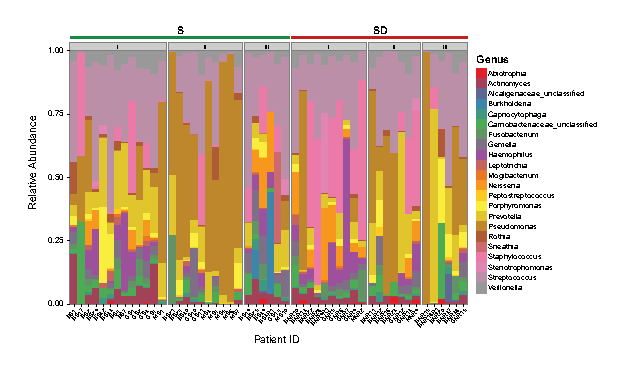
\includegraphics[width=1\textwidth]{./figures/Chapter_7/Figure_1_16s}
  	\caption{\label{fig:fig116s}Segmented bar plot reporting relative abundances of OTU counts collapsed at Genus taxonomy level. OTU counts were transformed to relative abundance by dividing the number of assigned sequences by the sample size. Each bar of this plot reports the relative abundance of all genera detected in a sample (patient). The bar colors represent the different genera detected.}
\end{figure}
When the bacterial distribution at genus level was analyzed in terms of prevalence and abundance between groups (Figure~\ref{fig:fig216s}), similar patterns in all groups (S vs. SD at different FEV\textsubscript{1} groupings) were found for genera belonging to \textit{Actinobacteria}, \textit{Bacteroidetes}, \textit{Firmicutes} and \textit{Fusobacteria}. On the contrary, genera belonging to \textit{Proteobacteria }showed a more variable pattern. In particular, \textit{Pseudomonas} assignments within the SD group showed a pattern of increasing prevalence and abundance following FEV\textsubscript{1} groups. In the S group, \textit{Pseudomonas} assignments showed high levels of prevalence and abundance in the group II of FEV\textsubscript{1} only.\\ 
\begin{figure}[!tb]
	\centering
	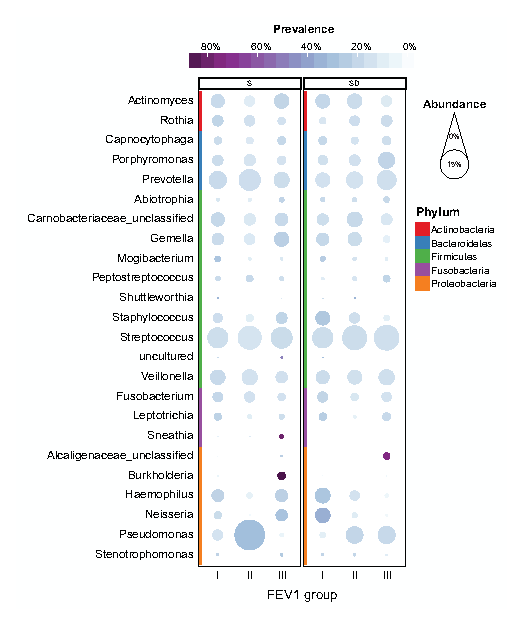
\includegraphics[width=0.7\textwidth]{./figures/Chapter_7/Figure_2_16s}
  	\caption{\label{fig:fig216s} Abundance and prevalence of detected taxa in CF patients. Prevalence (intensity of color) and abundance (size) of clades in the lung microbiome. Taxa belonging to the same Phylum were grouped together reporting a different color for each Phylum detected.}
\end{figure}

\subsubsection{Statistical evaluation of lung microbiota differences}
Rarefaction curves (Figure~\ref{fig:fig316s}) showed that all samples had the required amount of sequences to assess OTU richness (all curves reached an asymptote). After normalization of bacterial counts to relative abundance values, biodiversity indices have been calculated (Table SM3) and a two-factor Analysis of Variance (two-factor ANOVA) was carried out in order to evaluate if biodiversity values differed in relation to both patient status (S vs. SD) and pulmonary functionality (FEV\textsubscript{1} groups) (Table~\ref{tab:ffc216s}). 
\begin{figure}[!tb]
	\centering
	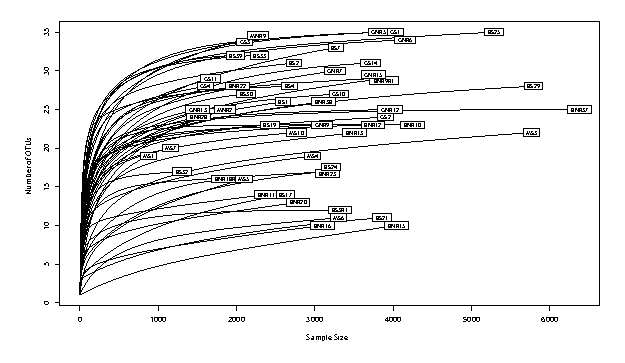
\includegraphics[width=0.8\textwidth]{./figures/Chapter_7/Figure_3_16s}
  	\caption{\label{fig:fig316s} Rarefaction curves calculated for sputum samples of all patients. A curve has been drawn for each sample with the sample ID reported at the end. As showed in this figure, all curves reached an asymptote whereas samples have not achieved the same number of sequences.}
\end{figure}
Regarding both Evenness and Shannon indices, the two-factor analysis of variance showed no significant effect for the single factors, but their interaction was significant. On the contrary, Richness index showed a significant effect of the FEV\textsubscript{1} index, but no significant effect between S and SD groups (Table~\ref{tab:ffc316s}). Furthermore, a Tukey's HSD test has been performed for each index showing significant differences between group I and group II of FEV\textsubscript{1}. In particular, for Richness index a significant difference has been found passing from group I to group II of FEV\textsubscript{1} level, whereas, both for Shannon and Evenness indices, a significant difference has been found but only considering values from the S group (Figure SM2 and Table SM4).\\
\begin{table}
\centering
\scriptsize
\begin{tabular}{ c c c c c c c c } 
\hline
FEV & Condition & \multicolumn{2}{c}{Richness} & \multicolumn{2}{c}{Shannon} & \multicolumn{2}{c}{Evenness}\\
\hline\hline
  &  & Mean & St. Dev. & Mean & St. Dev. & Mean & St. Dev. \\
I & S & 23.5512 & 6.1071 & 2.2006 & 0.4976 & 0.7010 & 0.1202 \\
I & SD & 23.4139 & 3.7107 & 1.8466 & 0.4816 & 0.5859 & 0.1447 \\
II & S & 16.3694 & 6.5919 & 1.3104 & 0.6641 & 0.4693 & 0.2103 \\
II & SD & 18.1791 & 8.2644 & 1.7579 & 0.5979 & 0.6162 & 0.1252 \\
III & S & 23.7927 & 5.1791 & 2.2185 & 0.3820 & 0.7014 & 0.0783 \\
III & SD & 16.2788 & 8.2847 & 1.4349 & 0.7957 & 0.5015 & 0.2590 \\
\hline
\end{tabular}
\caption{\label{tab:ffc216s}Biodiversity indices means and standard deviations for each group of patients.} 
\end{table}
Subsequently, a two-factor multivariate analysis of variance (MANOVA) was conducted considering OTUs as dependent variables. Likewise the ANOVA analysis described above, we have used the same factors FEV\textsubscript{1} and condition (S and SD) to test the hypothesis that there would be differences in OTU counts between these groups. The condition factor showed a statistically significant effect, Pillais' Trace = 0.99, F approx = 8.82, p {\textless} 0.05 (for additional information see Table SM5).\\
\begin{table}
\centering
\scriptsize
\begin{tabular}{ r c c c c c l}
  &  &  &  &  &  &  \\
a) \hfill \textbf{Richness} & Df & Sum Sq & Mean Sq & F value & Pr(>F) & \\
\hline\hline
FEV1 & 2 & 416.5000 & 208.2300 & 4.8360 & 0.0124 & * \\
Condition & 1 & 10.9000 & 10.8800 & 0.2530 & 0.6175 & \\
FEV1:Condition & 2 & 117.5000 & 58.7500 & 1.3650 & 0.2656 & \\
Residuals & 46 & 1980.6000 & 43.0600 &  &  & \\
\hline
  &  &  &  &  &  & \\
b) \hfill \textbf{Shannon} & Df & Sum Sq & Mean Sq & F value & Pr(>F) & \\
\hline\hline
FEV1 & 2 & 2.9820 & 1.4909 & 4.4560 & 0.0170 &  * \\
Condition & 1 & 0.4250 & 0.4250 & 1.2700 & 0.2656 & \\
FEV1:Condition & 2 & 2.6800 & 1.3399 & 4.0050 & 0.0249 & * \\
Residuals & 46 & 15.392 & 0.3346 &  &  & \\
\hline
  &  &  &  &  &  & \\
c) \hfill \textbf{Evenness} & Df & Sum Sq & Mean Sq & F value & Pr(>F) & \\
\hline\hline
FEV1 & 2 & 0.1431 & 0.0715 & 2.6980 & 0.0780 & \\
Condition & 1 & 0.0326 & 0.0326 & 1.2310 & 0.2731 & \\
FEV1:Condition & 2 & 0.2515 & 0.1257 & 4.7420 & 0.0134 & * \\
Residuals & 46 & 1.2197 & 0.0265 &  &  & \\
\hline
\end{tabular}
\caption{\label{tab:ffc316s}Two-factor Analysis of Variance (ANOVA) of biodiversity indices. As reported in the table for both Shannon (b) and Evenness (c) indices, the analysis has shown a statistically significant effect of the interaction between the two factors considered (FEV\textsubscript{1} index and patient condition). On the other hand, regarding Richness index (a), the analysis has shown a significant effect of the FEV\textsubscript{1} index only. Any P value less than 0.05 has been marked with an asterisk to signal a statistically significant variation between groups.} 
\end{table}
In order to further investigate the dependence of bacterial community composition from patient conditions we perform a constrained Canonical-Correlation Analysis (CCA) using log normalized OTU counts (Figure~\ref{fig:fig416s}). CCA analysis results showed that both FEV\textsubscript{1} and condition factors, included in the analysis, were able to explain 15 \% only of the total variance, suggesting that this two factors were not able to discriminate the major taxa detected. However, CCA1 and CCA2 together explained more than 73 \% of the constrained inertia, denoting these two coordinates as acceptable candidates to represent the CCA results. As shown in Figure 4, there is a high level of overlap between samples (the gray ellipse), but, despite the low level of variance explained by the constrained CCA analysis, samples from group III of FEV\textsubscript{1} index constitute two distinct clusters. One cluster included patients from the S group and the other one contained patients from the SD group.\\
\begin{figure}[!tb]
	\centering
	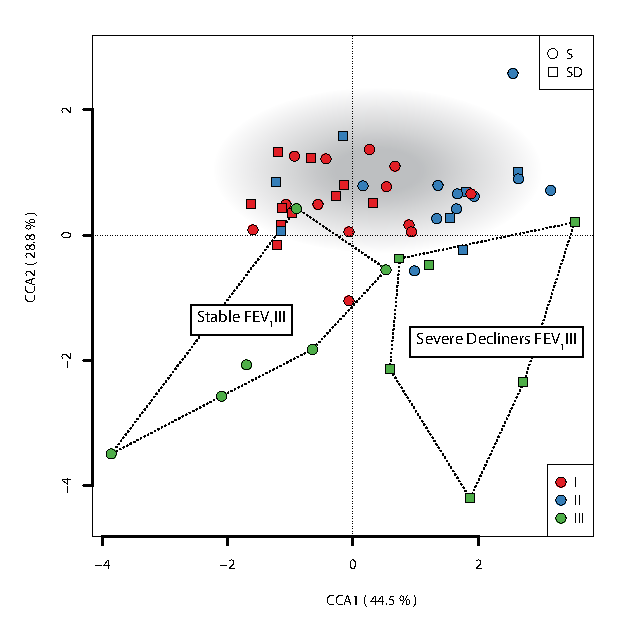
\includegraphics[width=0.7\textwidth]{./figures/Chapter_7/Figure_4_16s}
  	\caption{\label{fig:fig416s}Results of Canonical Correlation Analysis. The dot colors represent the level of the FEV1 index, whereas the dot shapes correspond to patient condition (S or SD). The grey area shows the section of the plot with the highest level of overlap; on the other hand, two clusters with low level of overlap were reported using a dotted line. These clusters contain all samples from the FEV\textsubscript{1} III group divided according to their condition (S or SD).}
\end{figure}

\subsubsection{Network analysis}
In order to evaluate the presence of different co-occurrence patterns of OTUs in patients with different status (S and SD), a network of correlations between OTUs was built. This approach has been widely used to successfully explore the interaction between organisms from different environments and to study the association between organisms and their environment \cite{barberan2011using, chaffron2010global}. The networks obtained from the OTU counts of S and SD patients consisted of 44 and 42 OTUs (nodes), respectively (Figure~\ref{fig:fig516s}). The number of links (vertices) of the two networks was 204 and 129, with the SD network containing 75 links less than the S one. Moreover, the S network (Figure~\ref{fig:fig516s} (a)) showed a higher level of interconnections between OTUs with an average degree value of 9.273, against a value of 6.143 of the SD network (Figure~\ref{fig:fig516s} (b)). It is worth of mentioning that bacteria belonging to \textit{Pseudomonas }genus (the blue node in Figure 5) were not linked with any other node in both S and SD. The same approach of network construction was used also to look at potential different patterns in relation to FEV\textsubscript{1} conditions in each status, but no clear differences were observed (Figure SM5).\\
\begin{figure}[!tb]
	\centering
	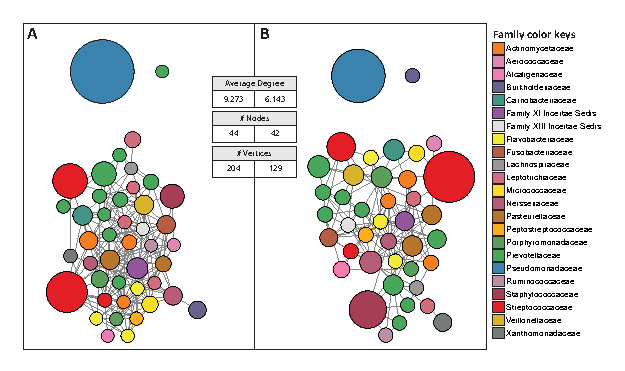
\includegraphics[width=1\textwidth]{./figures/Chapter_7/Figure_5_16s}
  	\caption{\label{fig:fig516s}OTU Networks based on correlation analysis. A connection between two OTUs (nodes) stand for a significant correlation between the two linked OTUs (Spearman's value {\textgreater} 0.6 and p-value {\textless} 0.05). The size of each node is proportional to the OTU count in the dataset. The two panels report the network representation of lung microbiota for both A) Stable and B) Severe decliner patients.}
\end{figure}

\subsection{Discussion}
During the last 5 years, the perspective of CF airway infection has changed from one based on the analysis of a single pathogen organism to one based on the analysis of the whole lung bacterial community. Several studies have shown that lung bacterial community is very heterogeneous and that this heterogeneity may vary with the age of patients \cite{cox2010airway, rogers2010determining, willner2009metagenomic, rogers2004characterization}. In this study we have inspected the sputum bacterial community of patients with different levels pulmonary functionality, aiming to find a correlation between the exacerbation of the CF disease and the variation in the bacterial community.\\
The 16S rRNA metabarcoding approach used, allowed to sample exhaustively the bacterial diversity (see Figure~\ref{fig:fig316s}) and showed the presence of 22 genera, mainly belonging to both \textit{Proteobacteria} (6 genera) and \textit{Firmicutes} (10 genera) phyla. Interestingly, the phylum showing the highest heterogeneity among S and SD patients and among FEV\textsubscript{1} groups was that of \textit{Proteobacteria, }which in our study was mainly represented by the genera traditionally recognized as CF pathogens (\textit{Haemophilus}, \textit{Pseudomonas}, \textit{Stenotrophomonas}, \textit{Burkholderia}) together with an unclassified genus of the \textit{Alcaligenaceae }family) \cite{lipuma2010changing}. These data allow concluding that indeed culture-based methods provide a good estimation of main taxa which colonize the lung of CF patients. However, since 16S rRNA metabarcoding does not allow defining species or strain identity, we cannot exclude the presence of new species, within those genera, as new opportunistic pathogens of CF patients.\\
Intriguing data were obtained from the analysis of bacterial community diversity and the influence of OTU distribution with respect to the conditions of the patients. Here, OTU distribution and OTU co-occurrence were clearly different between S and SD group. Moreover, when considering the FEV\textsubscript{1} conditions, most of the differences concerned FEV\textsubscript{1} I vs. FEV\textsubscript{1} II groups, for both S and SD patients (Richness) or for S patients only (both Shannon and Evenness indices).\\
Summarizing, our findings allow proposing a scheme of lung bacterial colonization patterns in relation to status (S and SD) and FEV\textsubscript{1} condition (Figure~\ref{fig:fig616s}). Stable patients showed a drop of lung microbiota biodiversity passing from group I to group II of FEV\textsubscript{1} index; we can speculate that between FEV textsubscript{1} I and FEV\textsubscript{1} II something (still unknown) is occurring in the ecology of lung bacterial communities, which may ultimately unbalance bacterial community ecology, opening the way to a more severe condition.\\
\begin{figure}[!tb]
	\centering
	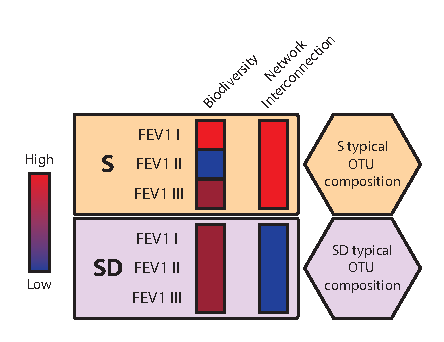
\includegraphics[width=0.6\textwidth]{./figures/Chapter_7/Figure_6_16s}
  	\caption{\label{fig:fig616s}Model of lung bacteria colonization. Two distinct patterns are reported for both S and SD patients showing diverging characteristics.}
\end{figure}
We can speculate, in an ecological perspective \cite{conrad2013cystic}, that a relatively complex bacterial community is present only in patients with a low level of disease (first group of FEV\textsubscript{1}), whereas, higher levels of pulmonary deficiency (in patients not under exacerbation, the S group), can lead to a drastic decrement of the lung bacterial community complexity leaving the way clear for the proliferation of pathogens bacteria (prevalence of diversity in members of  \textit{Proteobacteria} phylum).\\
As a consequence, we can advocate that bacterial lung microbiota is modified along with changes in CF patient conditions. In particular, as highlighted by network analysis, S patients have a more complex and interconnected lung microbiota than the SD ones. We can then hypothesize that the reduction of bacterial community connections may be due to a higher level of lung colonization from pathogenic bacteria (again the prevalence of members of \textit{Proteobacteria} phylum). This, in turn, may lead to a selection of opportunistic taxa with a lower positive correlation with the others. Here, the absence of correlation of \textit{Pseudomonas} representatives with the other detected OTUs could reinforce the role that members of this genus (e.g. \textit{P. aeruginosa}) may have in pulmonary damage.\\

%%-----------
%% Backmatter
%%-----------
\backmatter
\chaptermark{Bibliography}
\renewcommand{\sectionmark}[1]{\markright{#1}}
\bibliographystyle{unsrt}                           %Use alpha codes for references
\sectionmark{Bibliography}
\addcontentsline{toc}{chapter}{Bibliography}        %Force addition of Bibliography to TOC    
\bibliography{References}